%%% The main file. It contains definitions of basic parameters and includes all other parts.

%% Settings for single-side (simplex) printing
% Margins: left 40mm, right 25mm, top and bottom 25mm
% (but beware, LaTeX adds 1in implicitly)
\documentclass[12pt,a4paper]{report}
\setlength\textwidth{145mm}
\setlength\textheight{247mm}
\setlength\oddsidemargin{15mm}
\setlength\evensidemargin{15mm}
\setlength\topmargin{0mm}
\setlength\headsep{0mm}
\setlength\headheight{0mm}
% \openright makes the following text appear on a right-hand page
\let\openright=\clearpage

%% Settings for two-sided (duplex) printing
% \documentclass[12pt,a4paper,twoside,openright]{report}
% \setlength\textwidth{145mm}
% \setlength\textheight{247mm}
% \setlength\oddsidemargin{14.2mm}
% \setlength\evensidemargin{0mm}
% \setlength\topmargin{0mm}
% \setlength\headsep{0mm}
% \setlength\headheight{0mm}
% \let\openright=\cleardoublepage

%% Generate PDF/A-2u
\usepackage[a-2u]{pdfx}

%% Character encoding: usually latin2, cp1250 or utf8:
\usepackage[utf8]{inputenc}

%% Prefer Latin Modern fonts
\usepackage{lmodern}

%% Further useful packages (included in most LaTeX distributions)
\usepackage{amsmath}        % extensions for typesetting of math
\usepackage{amsfonts}       % math fonts
\usepackage{amsthm}         % theorems, definitions, etc.
\usepackage{bbding}         % various symbols (squares, asterisks, scissors, ...)
\usepackage{bm}             % boldface symbols (\bm)
\usepackage{dsfont}			% for indicator function
\usepackage{graphicx}       % embedding of pictures
\usepackage{fancyvrb}       % improved verbatim environment
\usepackage{natbib}         % citation style AUTHOR (YEAR), or AUTHOR [NUMBER]
\usepackage[nottoc]{tocbibind} % makes sure that bibliography and the lists
			    % of figures/tables are included in the table
			    % of contents
\usepackage{dcolumn}        % improved alignment of table columns
\usepackage{booktabs}       % improved horizontal lines in tables
\usepackage{paralist}       % improved enumerate and itemize
\usepackage{xcolor}         % typesetting in color
\usepackage{tablefootnote}

%%% Basic information on the thesis

% Thesis title in English (exactly as in the formal assignment)
\def\ThesisTitle{Neural Networks and Knowledge Distillation}

% Author of the thesis
\def\ThesisAuthor{Bc. Martin Grätzer}

% Year when the thesis is submitted
\def\YearSubmitted{2025}

% Name of the department or institute, where the work was officially assigned
% (according to the Organizational Structure of MFF UK in English,
% or a full name of a department outside MFF)
\def\Department{Department of Probability and Mathematical Statistics}

% Is it a department (katedra), or an institute (ústav)?
\def\DeptType{Department}

% Thesis supervisor: name, surname and titles
\def\Supervisor{Mgr. Ondřej Týbl, Ph.D.}

% Supervisor's department (again according to Organizational structure of MFF)
\def\SupervisorsDepartment{Department of Cybernetics, Faculty of Electrical Engineering, Czech Technical University in Prague}

% Study programme and specialization
\def\StudyProgramme{Financial and Insurance Mathematics}

% An optional dedication: you can thank whomever you wish (your supervisor,
% consultant, a person who lent the software, etc.)
\def\Dedication{%
I dedicate this thesis to all those who have supported me, mentally, financially, or academically, throughout my academic journey, of which this work represents the culmination.

I would like to express my gratitude to my thesis supervisor, Mgr. Ondřej Týbl, Ph.D., for his guidance, patience, and expert advice throughout the process. His feedback helped me see things more clearly and kept this work moving in the right direction. I really appreciate the time and effort he put into helping me finish this thesis.
}

% Abstract (recommended length around 80-200 words; this is not a copy of your thesis assignment!)
\def\Abstract{%
This thesis explores an enhancement to knowledge distillation by replacing Kullback-Leibler divergence with Rényi divergence, introducing a new hyperparameter for increased flexibility. To assess the effectiveness of this approach, it is tested on the CIFAR-100 dataset using the ResNet architecture. During testing three different approaches to the Rényi-based knowledge distillation has been formulated and compared, with the normalized version being the most promising. This work establishes a foundation for future research on the application of Rényi divergence in knowledge distillation.
}

% 3 to 5 keywords (recommended), each enclosed in curly braces
\def\Keywords{%
{neural networks} {machine learning} {knowledge distillation} {KL divergence}
}

% My own data
\def\ThesisTitleCS{Neuronové sítě a destilace znalostí}
\def\DepartmentCS{Katedra pravděpodobnosti a matematické statistiky}
\def\DeptTypeCS{Katedra}
\def\SupervisorsDepartmentCS{Katedra kybernetiky, Fakul\-ta elektrotechnická, České vysoké učení technické v Praze}
\def\StudyProgrammeCS{Finanční a pojistná matematika}

\def\ThesisKeywordsCS{%
	neuronové sítě\sep strojové učení \sep destilace znalostí \sep KL divergence
}

\def\AbstractCS{Tato práce zkoumá vylepšení metody destilace znalostí nahrazením Kullback-Leiblerovy divergence Rényiho divergencí, čímž zavádí nový hyperpara\-metr pro zvýšení flexibility. Pro posouzení účinnosti tohoto přístupu byla metoda testována na datasetu CIFAR-100 s využitím architektury ResNet. Během testo\-vá\-ní byly formulovány a porovnány tři různé přístupy k destilaci znalostí založené na Rényiho divergenci, přičemž nejperspektivnější se ukázala být normalizovaná verze. Tato práce vytváří základ pro budoucí výzkum aplikace Rényiho divergence v destilaci znalostí.}


%% The hyperref package for clickable links in PDF and also for storing
%% metadata to PDF (including the table of contents).
%% Most settings are pre-set by the pdfx package.
\hypersetup{unicode}
\hypersetup{breaklinks=true}

% Definitions of macros (see description inside)
%%% This file contains definitions of various useful macros and environments %%%
%%% Please add more macros here instead of cluttering other files with them. %%%

%%% Minor tweaks of style

% These macros employ a little dirty trick to convince LaTeX to typeset
% chapter headings sanely, without lots of empty space above them.
% Feel free to ignore.
\makeatletter
\def\@makechapterhead#1{
  {\parindent \z@ \raggedright \normalfont
   \Huge\bfseries \thechapter. #1
   \par\nobreak
   \vskip 20\p@
}}
\def\@makeschapterhead#1{
  {\parindent \z@ \raggedright \normalfont
   \Huge\bfseries #1
   \par\nobreak
   \vskip 20\p@
}}
\makeatother

% This macro defines a chapter, which is not numbered, but is included
% in the table of contents.
\def\chapwithtoc#1{
\chapter*{#1}
\addcontentsline{toc}{chapter}{#1}
}

% Draw black "slugs" whenever a line overflows, so that we can spot it easily.
\overfullrule=1mm

%%% Macros for definitions, theorems, claims, examples, ... (requires amsthm package)

\theoremstyle{plain}
\newtheorem{thm}{Theorem}
\newtheorem{lemma}[thm]{Lemma}
\newtheorem{claim}[thm]{Claim}

\theoremstyle{plain}
\newtheorem{defn}{Definition}

\theoremstyle{remark}
\newtheorem*{cor}{Corollary}
\newtheorem*{rem}{Remark}
\newtheorem*{example}{Example}

%%% An environment for proofs

\newenvironment{myproof}{
  \par\medskip\noindent
  \textit{Proof}.
}{
\newline
\rightline{$\qedsymbol$}
}

%%% An environment for typesetting of program code and input/output
%%% of programs. (Requires the fancyvrb package -- fancy verbatim.)

\DefineVerbatimEnvironment{code}{Verbatim}{fontsize=\small, frame=single}

%%% The field of all real and natural numbers
\newcommand{\R}{\mathbb{R}}
\newcommand{\N}{\mathbb{N}}

%%% Useful operators for statistics and probability
\DeclareMathOperator{\pr}{\textsf{P}}
\DeclareMathOperator{\E}{\textsf{E}\,}
\DeclareMathOperator{\var}{\textrm{var}}
\DeclareMathOperator{\sd}{\textrm{sd}}

%%% Transposition of a vector/matrix
\newcommand{\T}[1]{#1^\top}

%%% Various math goodies
\newcommand{\goto}{\rightarrow}
\newcommand{\gotop}{\stackrel{P}{\longrightarrow}}
\newcommand{\maon}[1]{o(n^{#1})}
\newcommand{\abs}[1]{\left|{#1}\right|}
\newcommand{\dint}{\int_0^\tau\!\!\int_0^\tau}
\newcommand{\isqr}[1]{\frac{1}{\sqrt{#1}}}

%%% Various table goodies
\newcommand{\pulrad}[1]{\raisebox{1.5ex}[0pt]{#1}}
\newcommand{\mc}[1]{\multicolumn{1}{c}{#1}}


% Title page and various mandatory informational pages
\begin{document}
%%% Title page of the thesis and other mandatory pages

%%% Title page of the thesis

\pagestyle{empty}
\hypersetup{pageanchor=false}
\begin{center}

\centerline{\mbox{
\includegraphics[width=166mm]{../img/logo-en.pdf}}}

\vspace{-8mm}
\vfill

{\bf\Large MASTER THESIS}

\vfill

{\LARGE\ThesisAuthor}

\vspace{15mm}

{\LARGE\bfseries\ThesisTitle}

\vfill

\Department

\vfill

{
\centerline{\vbox{\halign{\hbox to 0.45\hsize{\hfil #}&\hskip 0.5em\parbox[t]{0.45\hsize}{\raggedright #}\cr
Supervisor of the master thesis:&\Supervisor \cr
\noalign{\vspace{2mm}}
Study programme:&\StudyProgramme \cr
}}}}

\vfill

% Zde doplňte rok
Prague \YearSubmitted

\end{center}

\newpage

%%% Here should be a bound sheet included -- a signed copy of the "bachelor
%%% thesis assignment". This assignment is NOT a part of the electronic
%%% version of the thesis. DO NOT SCAN.

%%% A page with a solemn declaration to the bachelor thesis

\openright
\hypersetup{pageanchor=true}
\pagestyle{plain}
\pagenumbering{roman}
\vglue 0pt plus 1fill

\noindent
I declare that I carried out this master thesis on my own, and only with the cited
sources, literature and other professional sources.
I understand that my work relates to the rights and obligations under the Act No.~121/2000 Sb.,
the Copyright Act, as amended, in particular the fact that the Charles
University has the right to conclude a license agreement on the use of this
work as a school work pursuant to Section 60 subsection 1 of the Copyright~Act.

\vspace{10mm}

\hbox{\hbox to 0.5\hsize{%
In \hbox to 6em{\dotfill} date \hbox to 6em{\dotfill}
\hss}\hbox to 0.5\hsize{\dotfill\quad}}
\smallskip
\hbox{\hbox to 0.5\hsize{}\hbox to 0.5\hsize{\hfil Author's signature\hfil}}

\vspace{20mm}
\newpage

%%% Dedication

\openright

\noindent
\Dedication

\newpage

%%% Mandatory information page of the thesis

\openright

\vbox to 0.5\vsize{
\setlength\parindent{0mm}
\setlength\parskip{5mm}

Title:
\ThesisTitle

Author:
\ThesisAuthor

\DeptType:
\Department

Supervisor:
\Supervisor, \SupervisorsDepartment

Abstract:
\Abstract

Keywords:
\Keywords

\vss}

\vtop to 0.49\vsize{
\setlength\parindent{0mm}
\setlength\parskip{5mm}

Název práce:
\ThesisTitleCS

Autor:
\ThesisAuthor

\DeptTypeCS:
\DepartmentCS

Vedoucí diplomové práce:
\Supervisor, \SupervisorsDepartmentCS

Abstrakt:
\AbstractCS

Klíčová slova:
{\def\sep{\unskip, }\ThesisKeywordsCS}

\vfil
}

\newpage

\openright
\pagestyle{plain}
\pagenumbering{arabic}
\setcounter{page}{1}


%%% A page with automatically generated table of contents of the bachelor thesis

\tableofcontents

%%% Each chapter is kept in a separate file
\chapter*{Introduction}
\addcontentsline{toc}{chapter}{Introduction}

In the recent years we have experienced a remarkable surge in artificial intelligence (AI). This rise has been fueled by an increase in computational power, making the creation of more powerful and complex models feasible. However, when deploying a model to a large number of users, we are usually more stringent regarding latency, as well as computational and storage capacity. Yet, simply using a smaller model does not take full advantage of the training capacity we usually possess.

A proposed solution to these seemingly opposing constrains is knowledge distillation. This approach involves training a large model, known as the teacher, and transferring its knowledge to a smaller model, called student, we want to deploy. We believe that the teacher is able to better extract the structure from the data. It learns to differentiate between large number of classes and then correctly predict the label when exposed to new data. Additionally, the trained model also assigns weights to all of the possible classes, which are then converted into probabilities using a softmax function. Even though these are often very small for the incorrect answers, they can still provide valuable information about how the larger model generalizes.

For example, an image of a \textit{horse} will be correctly labeled by the teacher model with high probability close to 1. However, the model might also assign a small but nonzero probability that the image is a \textit{zebra}. We argue that this probability will still be many times higher than the probability assigned to an unrelated class, such as a \textit{car}.

Transferring this knowledge from the teacher to the student is done through distillation, where the student model is trained using the class probabilities produced by the teacher. In the original paper, the distillation process is formulated as the minimization of the Kullback–Leibler (KL) divergence.

In this work, we propose enhancing the distillation process by replacing the KL divergence with Rényi divergence, which serves as its generalization, and introduces an additional hyperparameter $\alpha$. We aim to formally define this new distillation framework, analyze the theoretical properties of Rényi-based distillation, and conduct experiments to evaluate the appropriateness of this approach.


\chapter{Rényi Divergence and Knowledge Distillation} 

In this chapter, we begin by examining the concepts of entropy, cross-entropy, and divergence. In particular, we define Rényi divergence, establish its connection to KL divergence, and inspect some of the theoretical properties stated in \cite{vanErvenHarremoës2012}. In the second part, we formally define the notion of knowledge distillation, as proposed in \cite{HintonVinyalsDean2015}, and inspect some of the theoretical results presented therein. Furthermore, we analyze how these results change when incorporating Rényi divergence into the distillation process.

\section{KL Divergence and Rényi Divergence}

The concept of entropy, as the amount of uncertainty regarding the outcome of an experiment, was introduced by \cite{Shannon1948}.

\begin{defn}
	The entropy of a probability distribution $P = (p_1,\ldots,p_n)$ is given by
	\begin{equation*}
		H(P) = -\sum_{i=1}^{n} p_i \log p_i,
	\end{equation*}
	where we adopt the convention that $0 \log 0 = 0$.
	\label{Entropy}
\end{defn}

\begin{example}
	Let $P$ be the probability distribution of a fair coin toss, i.e., $P = (\frac{1}{2},\frac{1}{2})$. The entropy $H(P)$ is approximately $0.693$. Next, let $Q$ represent the probability distribution of an unfair coin toss, i.e., $Q = (\frac{4}{10},\frac{6}{10})$. Here, the entropy $H(Q)$ is smaller than $H(P)$, approximately $0.673$. In other words, we are less uncertain about the outcome of the unfair coin toss than about the fair coin toss.
\end{example}

To determine the similarity between two probability distributions, we cannot simply subtract their entropies. For example, the entropy of $P_1 = (\frac{4}{10},\frac{6}{10})$ is the same as the entropy of $P_2 = (\frac{6}{10},\frac{4}{10})$, yet they represent different distributions. Therefore, we use the concept of divergence, as proposed by \cite{KullbackLeibler1951}. First, we define a related notion of cross-entropy.

\begin{defn}
	The cross-entropy of a probability distribution $P = (p_1,\ldots,p_n)$ relative to another distribution $Q = (q_1,\ldots,q_n)$ is given by
	\begin{equation*}
		H(P,Q) = -\sum_{i=1}^{n} p_i \log q_i,
	\end{equation*}
	where we adopt the convention that $0 \log 0 = 0$.
	\label{Cross-Entropy}
\end{defn}

\begin{example}
	Let $P$ and $Q$ be the probability distributions as described in the example above, i.e., $P = (\frac{1}{2},\frac{1}{2})$ and $Q = (\frac{4}{10},\frac{6}{10})$. The cross-entropy of $P$ relative to $Q$ is $H(P,Q) \approx 0.714$. On the other hand $H(Q,P) \approx 0.693$  and we observe that cross-entropy is not symmetric in its arguments.
\end{example}

\begin{defn}
	The Kullback–Leibler divergence (KL divergence) of a probability distribution $P = (p_1,\ldots,p_n)$ relative to another distribution $Q = (q_1,\ldots,q_n)$ is given by
	\begin{equation*}
		D_{\text{KL}}(P \| Q) = \sum_{i=1}^{n} p_i \log \frac{p_i}{q_i},
	\end{equation*}
	where we adopt the convention that $\frac{0}{0} = 0$ and $\frac{x}{0} = \infty$ for $x>0$.
	\label{KL Divergence}
\end{defn} 

We can decompose the KL divergence into two terms, as
\begin{equation}
	\begin{aligned}
		D_{\text{KL}}(P \| Q) =& \sum_{i=1}^{n} p_i \log \frac{p_i}{q_i} \\
		=& \sum_{i=1}^{n} p_i \log p_i  + \left( - \sum_{i=1}^{n} p_i \log q_i \right), \\
		=& - H(P) + H(P, Q)
	\end{aligned}
	\label{KL_decomposition}
\end{equation}
and we observe that cross-entropy can be decomposed into entropy and KL divergence.

\begin{example}
	Let $P$ and $Q$ be probability distributions, given as $P = (\frac{1}{2},\frac{1}{2})$ and $Q = (\frac{4}{10},\frac{6}{10})$. From the previous examples, we know that $H(P) \approx 0.693$ and $H(P,Q) \approx 0.714$. Using Equation~(\ref{KL_decomposition}), we can calculate the KL divergence of $P$ relative to $Q$ as $D_{\text{KL}}(P \| Q) = - H(P) + H(P, Q) \approx 0.021$.
\end{example}

Kullback–Leibler divergence was later generalized by \cite{Rényi1961}. We begin with the definition.

\begin{defn}
	The Rényi divergence of order $\alpha$ of a probability distribution $P = (p_1,\ldots,p_n)$ relative to another distribution $Q = (q_1,\ldots,q_n)$ is given by
	\begin{equation*}
		D_\alpha(P \| Q) = \frac{1}{\alpha-1} \log \sum_{i=1}^{n} p_i^\alpha q_i^{1-\alpha},
	\end{equation*}
	where $\alpha$ is positive number distinct from 1, and we adopt the convention that $\frac{0}{0} = 0$ and $\frac{x}{0} = \infty$ for $x>0$.
	\label{Rényi Divergence}
\end{defn}

This definition of Rényi divergence assumes that probability distributions $P$ and $Q$ are discrete. For continuous spaces we can substitute the sum by Lebesgue integral (see \cite{vanErvenHarremoës2012}). Now, we present an example that motivated the introduction of the normalization term $\frac{1}{\alpha-1}$ in the definition.

\begin{example}
	Let $Q$ be a probability distribution and $A$ be a set, such that $Q(A)>0$. Define $P$ as the conditional distribution of $Q$ given $A$, i.e. $P(x) = Q(x|A) = \frac{Q(x)}{Q(A)}$, for $x \in A$. Now compute the Rényi divergence of $P$ relative to $Q$
	
	\begin{align*}
		D_\alpha(P \| Q) &= \frac{1}{\alpha-1} \log \sum_{x\in A} P(x)^\alpha Q(x)^{1-\alpha}, \\
		&= \frac{1}{\alpha-1} \log \sum_{x\in A} \left(\frac{Q(x)}{Q(A)}\right)^\alpha Q(x)^{1-\alpha}, \\
		&= \frac{1}{\alpha-1} \log \sum_{x\in A} \frac{Q(x)}{Q(A)^\alpha}, \\
		&= \frac{1}{\alpha-1} \log \left( Q(A)^{-\alpha} \sum_{x\in A} Q(x) \right), \\
		&= \frac{1}{\alpha-1} \log Q(A)^{1-\alpha}, \\
		&= - \log Q(A).
	\end{align*}
	In this particular example we observe that the factor $\frac{1}{\alpha-1}$ in the definition of Rényi divergence has the effect that $D_\alpha(P \| Q)$ does not depend on $\alpha$ in this example. This factor is moreover crucial in the following consideration.
\end{example}

Definition~\ref{Rényi Divergence} was formulated for orders $\alpha \in (0,1) \cup (1,\infty)$. We now show that the limits on the borders of the domain for $\alpha$ exist and therefore Rényi divergence can be naturally extended to the cases $\alpha=0,1,\infty$. That is, we inspect the limits

\begin{align*}
	D_0(P \| Q) &= \lim_{\alpha \goto 0+} D_\alpha(P \| Q), \\
	D_1(P \| Q) &= \lim_{\alpha \goto 1} D_\alpha(P \| Q), \\
	D_\infty(P \| Q) &= \lim_{\alpha \goto \infty} D_\alpha(P \| Q).
\end{align*}
where $P$ and $Q$ are discrete distributions on $\{1,\dots,n\}$. For $\alpha = 0$, we have

\begin{equation}
\begin{aligned}
		\lim_{\alpha \goto 0+} D_\alpha(P \| Q) &= \lim_{\alpha \goto 0+} \frac{1}{\alpha-1} \log \sum_{i=1}^{n} p_i^\alpha q_i^{1-\alpha}, \\
		&= - \log \sum_{i=1}^{n} \lim_{\alpha \goto 0+} p_i^\alpha q_i^{1-\alpha}, \\
		&= - \log \sum_{i=1}^{n} q_i \lim_{\alpha \goto 0+} p_i^\alpha \\
		&= - \log \sum_{i=1}^{n} q_i \, \mathds{1}\{p_i>0\},
		\label{Rényi_0}
\end{aligned}
\end{equation}
where $\mathds{1}$ is the indicator function. For $\alpha = 1$, the limit

\begin{equation*}
	\lim_{\alpha \goto 1} \frac{1}{\alpha-1} \log \sum_{i=1}^{n} p_i^\alpha q_i^{1-\alpha}
\end{equation*}
is of an indeterminate form $\dfrac{0}{0}$, allowing us to apply L'Hopital's Rule and we obtain

\begin{equation}
	\begin{aligned}
		\lim_{\alpha \goto 1} \frac{1}{\alpha-1} \log \sum_{i=1}^{n} p_i^\alpha q_i^{1-\alpha} &= \lim_{\alpha \goto 1} \frac{\sum_{i=1}^{n} p_i^\alpha q_i^{1-\alpha} \log p_i - p_i^\alpha q_i^{1-\alpha} \log q_i}{\sum_{i=1}^{n} p_i^\alpha q_i^{1-\alpha}}, \\
		&= \frac{\sum_{i=1}^{n} p_i \log p_i - p_i \log q_i}{\sum_{i=1}^{n} p_i}, \\
		&= \sum_{i=1}^{n} p_i \log \frac{p_i}{q_i}.
	\end{aligned}
	\label{Rényi_1}
\end{equation}
Lastly, for $\alpha=\infty$, we denote $Z(\alpha) = \sum_{i=1}^{n} p_i^\alpha q_i^{1-\alpha}$, and $M = \max_{i} \frac{p_i}{q_i}$ and let $j \in \{1,\dots,n\}$ be the first index at which this maximum is attained. We have
\begin{equation}
	M^\alpha q_j \leq Z(\alpha) \leq M^\alpha \sum_{i=1}^{n} q_i.
	\label{M_Inequalities}
\end{equation}
Taking the logarithm and dividing by $\alpha-1$ preserves the inequalities, as the logarithm is a monotonic function and $\alpha > 1$. From (\ref{M_Inequalities}), we obtain that
\begin{equation*}
	  \frac{\alpha log M + \log q_j}{\alpha-1} \leq \frac{1}{\alpha-1} \log Z(\alpha)  \leq \frac{\alpha log M + \log 1}{\alpha-1}.
\end{equation*}
Taking the limit $\alpha \goto \infty$
%\begin{equation*}
	%\log M = \lim_{\alpha \goto \infty} \frac{\alpha log M + \log q_j}{\alpha-1} \leq \lim_{\alpha \goto \infty} \frac{1}{\alpha-1} \log Z(\alpha) \leq \lim_{\alpha \goto \infty} \frac{\alpha log M + \log 1}{\alpha-1} = \log M.
%\end{equation*}

\begin{align*}
	\log M &= \lim_{\alpha \to \infty} \frac{\alpha \log M + \log q_j}{\alpha - 1}, \\
	&\leq \lim_{\alpha \to \infty} \frac{1}{\alpha - 1} \log Z(\alpha), \\
	&\leq \lim_{\alpha \to \infty} \frac{\alpha \log M + \log 1}{\alpha - 1} = \log M.
\end{align*}

Thus,
\begin{equation}
	\begin{aligned}
		\lim_{\alpha \goto \infty} \frac{1}{\alpha-1} \log \sum_{i=1}^{n} p_i^\alpha q_i^{1-\alpha} = \lim_{\alpha \goto \infty} \frac{1}{\alpha-1} \log Z(\alpha) &= \log M, \\
		&= \max_{i} \log \frac{p_i}{q_i}.
	\label{Rényi_inf}
	\end{aligned}
\end{equation}
The limits (\ref{Rényi_0}), (\ref{Rényi_1}) , (\ref{Rényi_inf}) allow us to define the Rényi divergences
\begin{equation*}
	\begin{aligned}
		D_0(P \| Q) &= - \log \sum_{i=1}^{n} q_i \, \mathds{1}\{p_i>0\}, \\
		D_1(P \| Q) &= \sum_{i=1}^{n} p_i \log \frac{p_i}{q_i}, \\
		D_\infty(P \| Q) &= \max_{i} \log{\dfrac{p_i}{q_i}}.
	\end{aligned}
\end{equation*}
Comparing to Definition~\ref{KL Divergence}, we see that
\begin{equation*}
	D_1(P \| Q) = D_{\text{KL}}(P \| Q),
\end{equation*}
and Rényi divergence indeed generalizes KL divergence.

Another important case of Rényi divergence is for $\alpha=\frac{1}{2}$. For only this value the Rényi divergence is symmetric, i.e., $D_{1/2}(P \| Q) = D_{1/2}(Q \| P)$. Even with this additional property, it still does not satisfy the definition of a metric, as the triangle inequality does not hold. However, Rényi divergence of order $\frac{1}{2}$ can be rewritten as a function of the squared Hellinger distance, which, as defined in \cite{Cheng2024}, for discrete probability distributions $P$ and $Q$ is given by

\begin{equation*}
	H^2(P\|Q) = \frac{1}{2} \sum_{i=1}^{n} (p_i^\frac{1}{2} - q_i^\frac{1}{2})^2.
\end{equation*}
We also get a relation
\begin{equation*}
	\frac{1}{2} \sum_{i=1}^{n} (p_i^\frac{1}{2} - q_i^\frac{1}{2})^2 = \frac{1}{2} \left( \sum_{i=1}^{n} p_i + \sum_{i=1}^{n} q_i - 2 \sum_{i=1}^{n} p_i^\frac{1}{2} q_i^\frac{1}{2} \right) = 1 - \sum_{i=1}^{n} p_i^\frac{1}{2} q_i^\frac{1}{2},
\end{equation*}
which we can use in the definition of Rényi divergence of order $\frac{1}{2}$ to express it in terms of the Hellinger distance

\begin{equation*}
	D_{1/2}(P \| Q) = \frac{1}{\frac{1}{2}-1} \log \sum_{i=1}^{n} p_i^\frac{1}{2} q_i^{1-\frac{1}{2}} = - 2 \log (1-H^2(P\|Q)).
\end{equation*}

We can also establish a connection between Rényi divergence of order $\alpha$ and $1-\alpha$ for $0 < \alpha < 1$.

\begin{align*}
	D_{1-\alpha}(P \| Q) &= \frac{1}{-\alpha} \log \sum_{i=1}^{n} p_i^{1-\alpha} q_i^{\alpha}, \\
	&=\frac{1-\alpha}{\alpha} \left( \frac{\alpha}{1-\alpha}  \frac{1}{-\alpha} \log \sum_{i=1}^{n} q_i^{\alpha} p_i^{1-\alpha} \right), \\
	&= \frac{1-\alpha}{\alpha} D_{\alpha}(Q \| P).
\end{align*}

\begin{example}
	Let us have a probability distributions $Q = (\frac{4}{10},\frac{6}{10})$ and $P = (p,1-p)$ for some $p \in [0,1]$. On the left side of Figure~\ref{fig:renyi_divergence_example}, we plot $D_\alpha(P\|Q)$ as a function of $p$, for different values of $\alpha$. Clearly when $p=\frac{4}{10}$, the divergence is zero for any $\alpha$ since both distributions are identical. Additionally, the divergence remains the same for any $\alpha$, when $p=0$ or $p=1$. This follows from the fact that $D_\alpha(P\|Q) = \frac{1}{\alpha-1} \log q_1^{1-\alpha} = - \log q_1$ when $p=1$ and $D_\alpha(P\|Q) = - \log q_2$ when $p=0$.
	
	On the right side of Figure~\ref{fig:renyi_divergence_example}, we plot  $D_\alpha(P\|Q)$ as a function of $q$, where we now set $P = (\frac{4}{10},\frac{6}{10})$ and $Q = (q,1-q)$. Again, the divergence is always equal to zero, when the distributions are identical, e.g. when $q=\frac{4}{10}$. However, for $q=0$ or $q=1$, we obtain the expression $\frac{x}{0}$ for $x>0$, which as defined in Definition~\ref{Rényi Divergence}, is set to $\infty$ for $\alpha \in (0,1) \cap (1,\infty)$. Thus, the divergence is also $\infty$. For $\alpha = 1$, the divergence is also infinite, as follows from Definition~\ref{KL Divergence}.	Interestingly, for $\alpha=0$, from (\ref{Rényi_0}) we derive that the divergence is 0, which it is for any $q$. 
	
	For other values of $\alpha$, the divergence varies, but a clear ordering emerges. That is, in the first example, the value of $D_\alpha(P\|Q)$ for $\alpha > \beta$ is greater than or equal to $D_\beta(P\|Q)$ for any $p \in [0,1]$, this is also true for the second example for any $q \in [0,1]$. Moreover, as shown by \cite{vanErvenHarremoës2012}, this holds in general, as Rényi divergence is non-decreasing in $\alpha$.
	
	Additionally, in the first example, we observe that for larger values of $\alpha$ the derivative is greater when $p$ is close to $\frac{4}{10}$, whereas it is smaller when $p$ is near $0$ or $1$. The opposite holds for smaller values of $\alpha$. Conversely, for the second example, the derivative is high as we get near $0$ or $1$, actually it converges to infinity for $\alpha>0$. As shown in the figure, the rate of this convergence is slower for small values of $\alpha$.
	 
	\begin{figure}[h!]
		\centering
		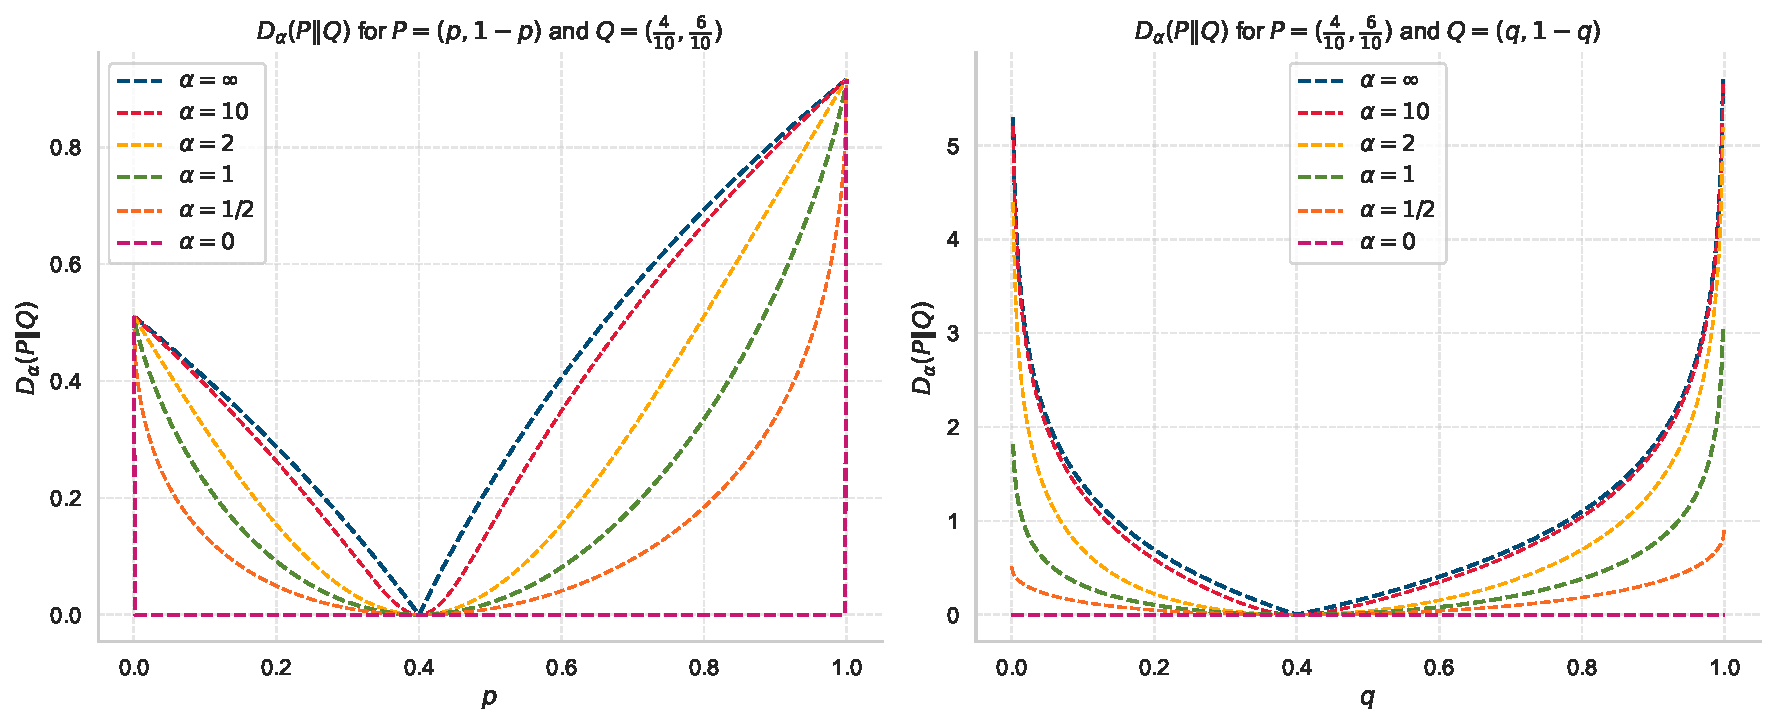
\includegraphics[width=0.9\textwidth]{../img/renyi_divergence_comparison.pdf}
		\caption{Example of Rényi divergence for a fixed distribution and another varying along the x-axis.}
		\label{fig:renyi_divergence_example}
	\end{figure}
\end{example}

The final property we focus on is the lower semi-continuity.

\begin{thm}
	Suppose we have a discrete sample space $\mathcal{Z} = \{z_1,z_2,z_3,\dots\}$ and sigma-algebra $\mathcal{A}$ is the power set of $\mathcal{Z}$. Then, for any order $\alpha \in (0,\infty]$, the Rényi divergence is a lower semi-continuous function of the pair $(P,Q)$ in the weak topology.
	\label{semicontinuity}
\end{thm}

\begin{proof}
	Let $P_1,P_2,\dots$ and $Q_1,Q_2,\dots$ be sequences of discrete distributions that weakly converge to $P$ and $Q$, respectively. We need to show
	\begin{equation*}
		\liminf_{n \goto \infty} D_\alpha(P_n \| Q_n) \geq D_\alpha(P \| Q).
	\end{equation*}
	Firstly, the weak convergence of discrete distribution $P$ means that for every bounded continuous function $h$
	\begin{equation*}
		\int h dP_n \goto \int h dP.
	\end{equation*}
	As the sample set is discrete, we may set $h=\mathds{1}\{z_i\}$ for any $i \in \N$, which is a bounded continuous function, and we obtain
	\begin{equation*}
		P_n(z_i) = \int \mathds{1}\{z_i\} dP_n \goto \int \mathds{1}\{z_i\} dP = P(z_i).
	\end{equation*}
	Now, any measurable set $A \in \mathcal{A}$ is just union of the individual elementary outcomes $z_i$  and thus the probability on any set $A$ is just the sum of the probabilities of the elementary outcomes. Using the convergence above we get
	\begin{equation*}
		P_n(A) = \sum_{z_i \in A} P_n(z_i) \goto \sum_{z_i \in A} P(z_i) = P(A),
	\end{equation*}
	and we proved that sequences $P_1,P_2,\dots$ and $Q_1,Q_2,\dots$ also converge pointwise to $P$ and $Q$, respectively. Thus, also the sequence of the pairs $(P_n,Q_n)$ converges pointwise to $(P,Q)$.
	
	Now, we can apply Fatou’s lemma term-by-term on the sum
	\begin{equation*}
		\liminf_{n \goto \infty} \sum_{i} P_n(z_i)^{\alpha} Q_n(z_i)^{1-\alpha} \geq \sum_{i} \liminf_{n \goto \infty} P_n(z_i)^{\alpha} Q_n(z_i)^{1-\alpha} \geq \sum_{i} P(z_i)^{\alpha} Q(z_i)^{1-\alpha}.
	\end{equation*}
	Taking the logarithm and scaling the by $\frac{1}{\alpha-1}$ preserves this inequality, thus yielding the lower semi-continuity of $D_\alpha(P \| Q)$.
	
\end{proof}



\section{Knowledge Distillation}

Let us define a machine learning model as a function that maps input data to output predictions

\begin{equation*}
	f_{\theta}: \mathcal{X} \goto \mathcal{Z}
\end{equation*}
where $\mathcal{X}$ is the input space, $\mathcal{Z}$ is the output space and $\theta$ is a vector representing the set of parameters of the model. In our case, as input, the model receives images from $\mathcal{X}$, where each image is represented as a tensor in $\R^{h \times w \times c}$, where $h$ and $w$ denote the height and width in pixels, respectively, and $c$ represents the number of channels, where for RGB images $c = 3$. We assume a classification task with $n$ classes, i.e., $\mathcal{Z} = \R^{n}$, so the model outputs a vector of $n$ real-valued scores, referred to as logits, given by

\begin{equation*}
	z = f_\theta(x)
\end{equation*}
for $x \in \mathcal{X}$. To convert these logits into probabilities, we use the softmax function, which is defined as

\begin{equation}
	\sigma(s)_k = \frac{e^{s_k}}{\sum_{i=1}^{n} e^{s_i}}, \qquad k = 1,2,\dots, n,
	\label{softmax}
\end{equation}
where $s \in \mathcal{Z}$. Now let

\begin{equation*}
	q_k = \sigma(z)_k, \qquad k = 1,2,\dots, n,
\end{equation*}
which represents the probability that $x$ belongs to class $k$. We denote the probability distribution produced by the model $f_\theta$ as $Q=\left(q_1,q_2,\dots,q_n\right)$. We denote by $\mathcal{Y}$ the space of such distributions, that is, $\mathcal{Y} = \{ y \in \R^n \mid y_k \geq 0 \text{ for all } k, \sum_{k=1}^{n} y_k = 1\}$. Hence, the model output $Q \in \mathcal{Y}$.

Additionally, a hyperparameter $T$, called temperature, is introduced to control the entropy of the output distribution. That is we set for $T>0$

\begin{equation}
	q_k^T = \sigma \left( \frac{z}{T} \right)_k, \qquad k = 1,2,\dots, n.
    \label{logits student}
\end{equation}
The produced probability distribution is $Q^T=\left(q^T_1,q^T_2,\dots,q^T_n\right)$. The process in called temperature scaling and popular choices for $T$ according to \cite{ChoHariharan2019} are 3, 4 and 5. Clearly, $Q^1 = Q$.

\begin{example}
	Following the example from the introduction, suppose a model $f_\theta$ that for given input yields logits for the classes \textit{horse}, \textit{zebra}, and \textit{car}, equal to 5.4, 0.2, and -1.3 respectively. In Figure~\ref{fig:temperature_example}, we see the logit values in a bar chart, along with the computed probabilities using the softmax function, both without and with temperature scaling, the latter corresponding to $T=4$.
	
	Without temperature scaling, the model is highly confident that the input belongs to the class \textit{horse} ($>0.99$), while the probabilities for the remaining classes are essentially zero. We observe that the effect of the temperature scaling is that the model is less confident about the true label while the order of the class probabilities in maintained.
	
	\begin{figure}[h!]
		\centering
		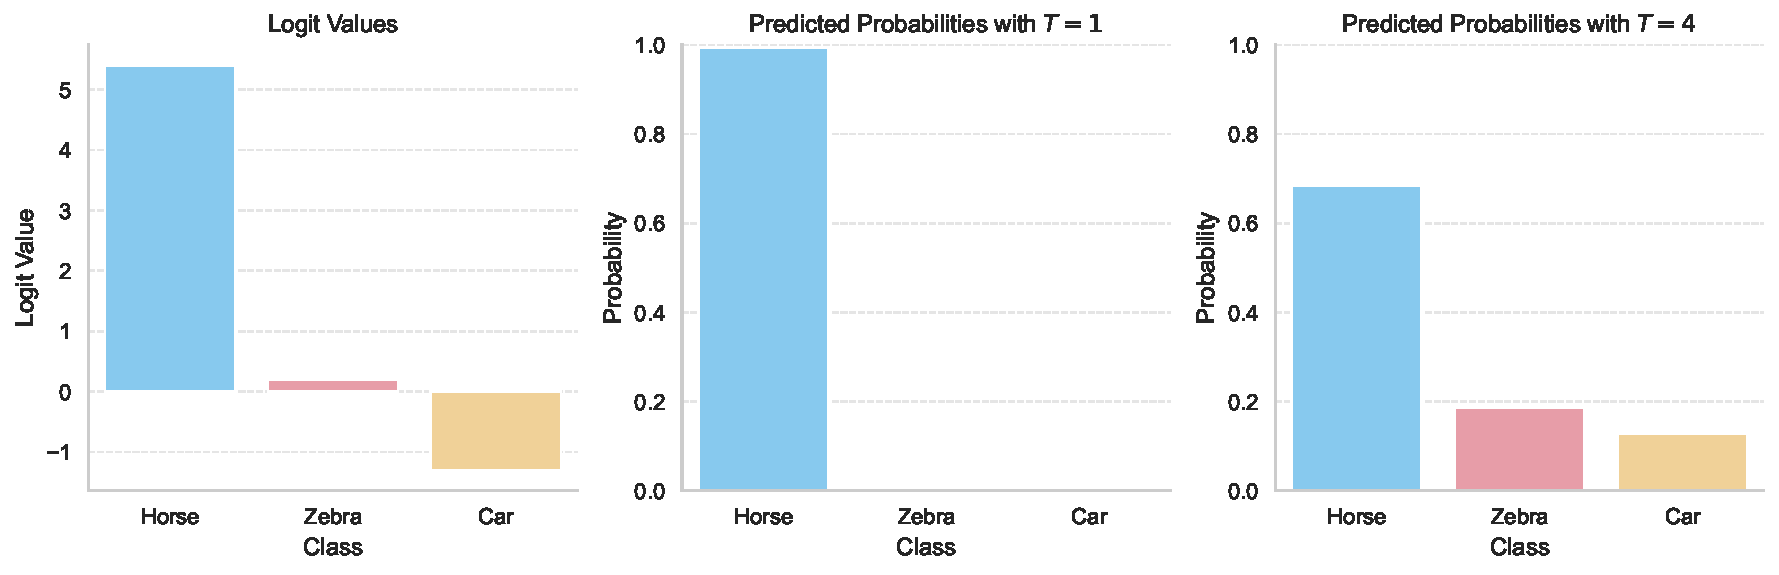
\includegraphics[width=0.9\textwidth]{../img/temperature_example_plot.pdf}
		\caption{Example of temperature scaling.}
		\label{fig:temperature_example}
	\end{figure}
\end{example}

Let $\mathcal{D}(x,y)$ denote a joint probability distribution over $\mathcal{X} \times \mathcal{Y}$, where $\mathcal{Y} = \R^n$, from which data points $(x,y)$ are independently and identically distributed (i.i.d.) samples. Now, the cross-entropy loss function $\mathcal{L_{\text{CE}}}$ is defined by

\begin{equation}
	\mathcal{L_{\text{CE}}}(\theta,x,y) = H(y \| Q) = - \sum_{j=1}^{n} y_{j} \log q_j,
	\label{Cross-entropy loss function}
\end{equation}
where $Q = (q_1,q_2,\dots,q_n)$ is the probability distribution obtained by applying the softmax function to the model's output $f(x)$, and $y_j$ is the one-hot ground-truth label, i.e., $y \in \mathcal{Y}$.

Although KL divergence provides a more intuitive measure of the difference between two distributions, being zero when the distributions are equal, unlike cross-entropy, we did not use it in Equation~(\ref{Cross-entropy loss function}). As shown in Equation~(\ref{KL_decomposition}), $H(P)$ does not depend on $Q$. Thus, the derivative of $D_{\text{KL}}(P \| Q)$ with respect to $Q$ is equal to the derivative of $H(P \| Q)$. Moreover, since cross-entropy is computationally simpler, especially when $P$ represents one-hot labels, it is often preferred over KL divergence in machine learning applications.

Training model $f_\theta$ is the process of finding the parameters $\theta$ that minimize the expected loss with respect to the distribution $\mathcal{D}$. That is, we want to find $\theta^*$ such that

\begin{equation}
	\theta^* = \arg \min_\theta \E_{(x,y) \sim \mathcal{D}} \mathcal{L_{\text{CE}}}(\theta,x,y).
	\label{vanilla_training}
\end{equation}

\begin{rem}
	In our context, the training process defined in Equation~(\ref{vanilla_training}) is referred to as vanilla training. This serves as a benchmark against which we compare our results.
\end{rem}

Knowledge distillation is a training technique where a smaller, so called student, model $f_\theta$ is trained to mimic a larger, so called teacher, model $f_t$, which has already been pre-trained. We now give a full definition.

\begin{defn}
	Suppose two models $f_\theta$ and $f_t$. Let $\mathcal{D}(x,y)$ denote a joint probability distribution over $\mathcal{X} \times \mathcal{Y}$, where $\mathcal{Y} = \R^n$, and $(x,y) \sim \mathcal{D}$. Also denote the outputs logits $z=f_\theta(x)$, which are converted into probability distribution $Q^T = (q^T_1,\dots,q^T_n)$ using softmax function introduced in Equation~(\ref{softmax}),
	\begin{equation*}
		q^T_k = \sigma \left( \frac{z}{T} \right)_k = \frac{e^\frac{z_k}{T}}{\sum_{i=1}^{n} e^\frac{z_i}{T}}, \qquad k = 1,2,\dots, n.
	\end{equation*}
	Similarly, the outputs logits $v=f_t(x)$, which are converted into probability distribution $P^T = (p^T_1,\dots,p^T_n)$ using softmax function,
	\begin{equation*}
		p^T_k = \sigma \left( \frac{v}{T} \right)_k = \frac{e^\frac{v_k}{T}}{\sum_{i=1}^{n} e^\frac{v_i}{T}}, \qquad k = 1,2,\dots, n.
	\end{equation*}
	Knowledge distillation of $f_\theta$ from $f_t$ is a training procedure in form of a minimization problem
	\begin{equation*}
		\theta^* = \arg \min_\theta \E_{(x,y) \sim \mathcal{D}} \mathcal{L}(\theta,x,y),
	\end{equation*}
	where
	\begin{equation}
		\mathcal{L}(\theta,x,y) = (1-\beta) \mathcal{L}_{\text{CE}}(\theta,x,y) + \beta \mathcal{L}_{\text{KL}}(\theta,x,y),
		\label{Knowledge Distillation Loss Function}
	\end{equation}
	where $\mathcal{L}_{\text{CE}}(\theta,x,y)$ is the standard cross-entropy loss with ground truth labels
	\begin{equation}
		\begin{aligned}
			\mathcal{L}_{\text{CE}}(\theta,x,y) &= H(y \| Q), \\
			&= - \sum_{j=1}^{n} y_{j} \log q_j,
			\label{CE loss}
		\end{aligned}
	\end{equation}
	and $\mathcal{L}_{\text{KL}}(\theta,x,y)$ is the Kullback-Leibler divergence loss with teacher's predictions
	\begin{equation}
		\begin{aligned}
			\mathcal{L}_{\text{KL}}(\theta,x,y) &= T^2 D_{\text{KL}}(P^T \| Q^T), \label{KL loss}\\
			&= T^2 \sum_{j=1}^{n} p^T_j \log \frac{p^T_j}{q^T_j},
		\end{aligned}
	\end{equation}
	$T$ and $\beta$ are hyperparameters.
	\label{Knowledge Distillation}
\end{defn}

The hyperparameter $T$ in Definition~\ref{Knowledge Distillation}  denotes temperature. During training, we apply temperature scaling to both the teacher and the student in Equation~(\ref{KL loss}). By increasing $T$, we soften the probabilities, thus retaining inter-class similarities by driving the predictions away from 0 and 1. The second hyperparameter, $\beta$, controls the balance between the cross-entropy loss and Kullback-Leibler divergence loss. A common choice for $\beta$ is $0.9$ (see \cite{ChoHariharan2019}).

%\begin{rem}
	%In many cases, the teacher model $f_t$ from Definition~\ref{Knowledge Distillation}, has been pre-trained on the same dataset $\mathcal{D}$. However, this is not always the case, for example, the teacher model may be trained on a much broader dataset or one that contains many more classes.
%\end{rem}

\begin{rem}
    The loss function in Equation~(\ref{KL loss}) includes a normalization term $T^2$, which we now elaborate on. First, we compute the derivative of the Kullback-Leibler divergence with respect to the logits of $Q^T:$
    \begin{equation}
	\begin{aligned}
		\frac{\partial D_\text{KL}(P^T \| Q^T)}{\partial z_j} &= \frac{\partial H(P^T \| Q^T)}{\partial z_j}\\
        &= - \frac{\partial}{\partial z_j}\left(\sum_{i=1}^{n} p^T_i \log \frac{e^{\frac{z_i}{T}}}{\sum_{k=1}^n e^{\frac{z_k}{T}}}\right)\\
		&= \left( \sum_{i=1}^{n} p^T_i \right)\frac{\partial}{\partial z_j}\left(\log \sum_{k=1}^n e^{\frac{z_k}{T}}\right) - \frac{\partial}{\partial z_j}\left(\sum_{i=1}^{n} p^T_i \frac{z_i}{T}\right) \\
		&= \frac{1}{T} \frac{e^{z_j}}{\sum_{k=1}^n e^{z_k}} - \frac{p^T_j}{T} \\
		&= \frac{1}{T} (q^T_j - p^T_j)
	\end{aligned}
    \label{KL gradient}
\end{equation}
If we now similarly to \cite{HintonVinyalsDean2015} assume centered logits
\begin{align}
\sum_{k=1}^{n} z_k = \sum_{k=1}^{n} v_k = 0,
    \label{centered logits}
\end{align}
we obtain by using a Taylor polynomial of order one for the exponential function
\begin{equation}
\begin{aligned}
    \frac{\partial D_\text{KL}(P^T \| Q^T)}{\partial z_j} &= \frac{1}{T} (q^T_j - p^T_j)\\
        &=\frac{1}{T} \left( \frac{e^{\frac{z_j}{T}}}{\sum_{k=1}^{n} e^{\frac{z_k}{T}}} - \frac{e^{\frac{v_j}{T}}}{\sum_{k=1}^{n} e^{\frac{v_k}{T}}} \right)\\
        &\approx \frac{1}{T} \left( \frac{1+{\frac{z_j}{T}}}{n + \sum_{k=1}^{n} {\frac{z_k}{T}}} - \frac{1+{\frac{v_j}{T}}}{n + \sum_{k=1}^{n} {\frac{v_k}{T}}} \right)\\
        &=\frac{1}{n T^2} (z_j-v_j).
\end{aligned}
	\label{additional term 1}
\end{equation}
We see that the Kullback-Leibler divergence gradient scales proportionally to $\frac{1}{T^2}$ with changing temperature $T$. Thus, we have incorporated the term $T^2$ into Equation~(\ref{KL loss}) to ensure that the relative contribution of $\mathcal{L}_{\text{CE}}(\theta,x,y)$ and $\mathcal{L}_{\text{KL}}(\theta,x,y)$ remains the same with changing temperature $T$. We also note that the approximation in Equation~(\ref{additional term 1}) is inaccurate when the temperature is small compared to the logits $z_k, v_k$. In that case, \cite{HintonVinyalsDean2015} states that the distillation pays less attention to matching logits much more negative than average. This is advantageous, as they may be significantly noisier, given that the teacher model is not penalized for them during training. On the other hand, they might convey useful information about the knowledge acquired by the teacher. Based on empirical evidence, the authors claim that ignoring large negative logits has a positive effect, as intermediate temperatures yield the best results.
\end{rem}

Now, we replace the KL divergence loss in knowledge distillation by a general Rényi divergence of order $\alpha$. 

\begin{defn}
    Assume the same setting as in Definition \ref{Knowledge Distillation}. Knowledge distillation with Rényi divergence of order $\alpha\in [0,\infty]$ is a training procedure as in Definition \ref{Knowledge Distillation} where the loss function~(\ref{Knowledge Distillation Loss Function}) is replaced by
    \begin{equation}
	\mathcal{L}(\theta,x,y) = (1-\beta) \mathcal{L}_{\text{CE}}(\theta,x,y) + \beta \mathcal{L}_{\alpha}(\theta,x,y),
	\label{Rényi Knowledge Distillation}
\end{equation}
where
\begin{equation}
	\begin{aligned}
		\mathcal{L}_{\alpha}(\theta,x,y) &= \frac{T^2}{\alpha} D_\alpha(P^T \| Q^T),\\
		&=\frac{T^2}{\alpha} \sum_{j=1}^{n} \frac{1}{\alpha-1} \log (p^T_j)^\alpha (q^T_j)^{1-\alpha}.
	\end{aligned}
	\label{Rényi loss}
\end{equation}
\end{defn}

\begin{rem}
    Similarly to above we elaborate on the normalizing factor in Equation~(\ref{Rényi loss}), which is now equal to $\frac{T^2}{\alpha}$. Our aim is to compute the derivatives of $D_{\alpha}(P^T \| Q^T)$ with respect to the logits of $Q^T$ for $\alpha\notin \lbrace 0,1,\infty\rbrace$ and to derive an analogous expression to Equation~(\ref{additional term 1})\footnote{Similar results as below hold to the remaining cases $\alpha\notin \lbrace 0,1,\infty\rbrace$ and can be shown using limiting procedures.}. First, recall the relation of the logits $z_k$ and probabilities $q_k$ in Equation~(\ref{logits student}) and denote
    \begin{equation*}
        Z_\alpha = \sum_{i=1}^{n} p_i^\alpha q_i ^{1-\alpha} = \sum_{i=1}^{n} p_i^\alpha \left( \frac{e^\frac{z_i}{T}}{\sum_{k=1}^n e^\frac{z_k}{T}} \right) ^{1-\alpha},
    \end{equation*}
    where we for simplicity omit $T$ in $P^T, Q^T, p^T$ and $q^T$. Now we calculate $\frac{\partial Z_\alpha}{\partial z_j}$:
\begin{align*}
	\frac{\partial Z_\alpha}{\partial z_j} =& \frac{\partial}{\partial z_j} \sum_{i=1}^{n} p_i^\alpha \left( \frac{e^\frac{z_i}{T}}{\sum_{k=1}^n e^\frac{z_k}{T}} \right) ^{1-\alpha}, \\
	=& \frac{\partial}{\partial z_j} p_j^\alpha \left( \frac{e^\frac{z_j}{T}}{\sum_{k=1}^n e^\frac{z_k}{T}} \right)^{1-\alpha} + \frac{\partial}{\partial z_j} \sum_{i\neq j}^{n} p_i^\alpha \left( \frac{e^\frac{z_i}{T}}{\sum_{k=1}^n e^\frac{z_k}{T}} \right) ^{1-\alpha}, \\
	=& p_j^\alpha (1-\alpha) \left( \frac{e^\frac{z_j}{T}}{\sum_{k=1}^n e^\frac{z_k}{T}} \right)^{-\alpha} \frac{\frac{1}{T} \sum_{k=1}^n e^\frac{z_k}{T} e^\frac{z_j}{T} - \frac{1}{T} e^\frac{z_j}{T} e^\frac{z_j}{T}}{(\sum_{k=1}^n e^\frac{z_k}{T})^2} \\
	& \qquad \qquad - \sum_{i\neq j}^{n} p_i^\alpha \left( \frac{e^\frac{z_i}{T}}{\sum_{k=1}^n e^\frac{z_k}{T}} \right)^{-\alpha} (1-\alpha) \frac{e^\frac{z_i}{T}}{(\sum_{k=1}^n e^\frac{z_k}{T})^2} e^\frac{z_j}{T} \frac{1}{T}, \\
	=& \frac{1-\alpha}{T} \left[ p_j^\alpha \left( \frac{e^\frac{z_j}{T}}{\sum_{k=1}^n e^\frac{z_k}{T}} \right)^{1-\alpha} \frac{\sum_{k=1}^n e^\frac{z_k}{T} - e^\frac{z_j}{T}}{\sum_{k=1}^n e^\frac{z_k}{T}} \right. \\
	& \qquad \qquad \left. - \sum_{i\neq j}^{n} p_i^\alpha \left( \frac{e^\frac{z_i}{T}}{\sum_{k=1}^n e^\frac{z_k}{T}} \right)^{1-\alpha} \frac{e^\frac{z_j}{T}}{\sum_{k=1}^n e^\frac{z_k}{T}} \right], \\
	=& \frac{1-\alpha}{T} \left[ p_j^\alpha q_j^{1-\alpha} (1-q_j) - \sum_{i\neq j}^{n} p_i^\alpha q_i^{1-\alpha} q_j \right], \\
	=& \frac{1-\alpha}{T} \left[ p_j^\alpha q_j^{1-\alpha} - q_j \sum_{i=1}^{n} p_i^\alpha q_i^{1-\alpha} \right], \\
	=& \frac{1-\alpha}{T} \left( p_j^\alpha q_j^{1-\alpha} - q_j Z_\alpha\right).
 \end{align*}
 By the chain rule and the shape of $\frac{\partial Z_\alpha}{\partial z_j}$ we have
\begin{equation}
\begin{aligned}
    \frac{\partial D_\alpha(P \| Q)}{\partial z_j}&= \frac{\partial}{\partial z_j} \left(\frac{1}{\alpha-1} \log \sum_{i=1}^{n} p_i^\alpha q_i ^{1-\alpha}\right)\\
    &=\frac{1}{\alpha-1}\frac{\partial}{\partial z_j}\left(\log Z_\alpha\right)\\
    &=\frac{1}{\alpha-1} \frac{1}{Z_\alpha} \frac{\partial Z_\alpha}{\partial z_j}\\
    &=\frac{1}{\alpha-1} \frac{1}{Z_\alpha}\frac{1-\alpha}{T}\left( p_j^\alpha q_j^{1-\alpha} - q_j Z_\alpha\right)\\
    &=\frac{1}{T} \left( q_j - \frac{p_j^\alpha q_j^{1-\alpha}}{\sum_{i=1}^{n} p_i^\alpha q_i^{1-\alpha}} \right)
\end{aligned}
\label{Rényi gradient}
\end{equation}
Using the formulas for logits of $p_j$ and $q_j$ we obtain
\begin{equation}
\begin{aligned}
    \frac{\partial D_\alpha(P \| Q)}{\partial z_j} &= \frac{1}{T} \left( q_j - \frac{p_j^\alpha q_j^{1-\alpha}}{\sum_{i=1}^{n} p_i^\alpha q_i^{1-\alpha}} \right)\\
    &=\frac{1}{T} \left[ \frac{e^{\frac{z_j}{T}}}{\sum_{k=1}^{n} e^{\frac{z_k}{T}}} -  \left( \frac{e^{\frac{v_j}{T}}}{\sum_{k=1}^{n} e^{\frac{v_k}{T}}} \right)^\alpha \left( \frac{e^{\frac{z_j}{T}}}{\sum_{k=1}^{n} e^{\frac{z_k}{T}}} \right)^{1-\alpha} \right. \\
    & \qquad \qquad \left. \left( \sum_{i=1}^{n} \left( \frac{e^{\frac{v_i}{T}}}{\sum_{k=1}^{n} e^{\frac{v_k}{T}}} \right)^\alpha \left( \frac{e^{\frac{z_i}{T}}}{\sum_{k=1}^{n} e^{\frac{z_k}{T}}} \right)^{1-\alpha} \right)^{-1} \right]
\end{aligned}
\label{complicated formula}
\end{equation}
Now we use an approximation by a Taylor polynomial of degree one. For that, we assume
\begin{align}
    \left(\frac{v_j}{T}\right)^2, \left(\frac{z_j}{T}\right)^2,\frac{v_jz_j}{T^2} \quad \text{are negligible} \quad j=1,\dots,n.
    \label{assumption negligible}
\end{align}
We also we suppose centered logits as in Equation~(\ref{centered logits}). We derive from (\ref{complicated formula}) and (\ref{assumption negligible})
\begin{align*}
	\frac{\partial D_\alpha(P \| Q)}{\partial z_j}\approx & \frac{1}{T} \left[ \frac{1+{\frac{z_j}{T}}}{n + \sum_{k=1}^{n} {\frac{z_k}{T}}} - \frac{1+{\frac{\alpha v_j}{T}}}{\left( n + \sum_{k=1}^{n} {\frac{v_k}{T}}\right)^\alpha} \frac{1+{\frac{(1-\alpha) z_j}{T}}}{\left( n + \sum_{k=1}^{n} {\frac{z_k}{T}}\right)^{1-\alpha}} \right. \\
	& \qquad \qquad \left. \left( \sum_{i=1}^{n} \frac{1+{\frac{\alpha v_i}{T}}}{\left( n + \sum_{k=1}^{n} {\frac{v_k}{T}}\right)^\alpha} \frac{1+{\frac{(1-\alpha) z_i}{T}}}{\left( n + \sum_{k=1}^{n} {\frac{z_k}{T}}\right)^{1-\alpha}} \right)^{-1} \right], \\
	=& \frac{1}{T} \left[ \frac{1+\frac{z_j}{T}}{n} - \frac{1 + \frac{\alpha v_j}{T} + \frac{(1-\alpha) z_j}{T} + \frac{\alpha (1-\alpha) v_j z_j}{T^2}}{n} \right. \\
	& \qquad \qquad \left. \left( \frac{1}{n} \sum_{i=1}^{n} 1 + \frac{\alpha v_i}{T} + \frac{(1-\alpha) z_i}{T} + \frac{\alpha (1-\alpha) v_i z_i}{T^2} \right)^{-1} \right]\\
    \approx& \frac{1}{T} \left[ \frac{1+\frac{z_j}{T}}{n} - \frac{1 + \frac{\alpha v_j}{T} + \frac{(1-\alpha) z_j}{T}}{n}\left( \frac{1}{n} \sum_{i=1}^{n} 1 + \frac{\alpha v_i}{T} + \frac{(1-\alpha) z_i}{T}\right)^{-1} \right]\\
    =&\frac{1}{T} \left[ \frac{1+\frac{z_j}{T}}{n} - \frac{1 + \frac{\alpha v_j}{T} + \frac{(1-\alpha) z_j}{T}}{n}\right]\\
    =&\frac{\alpha}{nT^2} (z_j - v_j).
\end{align*}
We have obtained
\begin{align*}
    \frac{\partial D_\alpha(P \| Q)}{\partial z_j}\approx\frac{\alpha}{nT^2} (z_j - v_j),
\end{align*}
which is a consistent formula to the case of KL divergence in (\ref{additional term 1}) which corresponds to $\alpha=1$. Also, the normalization term $\frac{\alpha}{T^2}$ in Equation~(\ref{Rényi loss}) was introduced so that the relative contribution of both terms in Equation~(\ref{Rényi Knowledge Distillation}) remains the same with changing the temperature $T$ and Rényi divergence parameter $\alpha$.
\end{rem}

\begin{rem}
If the distribution $P$ represents one-hot labels, that is $p_i=1$ for some $i\in\lbrace 1,\dots n\rbrace$, the derivative $\frac{\partial D_\alpha(P \| Q)}{\partial z_j}$ simplifies to the same form as in Equation~(\ref{KL gradient}). This holds for any choice of $\alpha$, which is why we do not modify the $\mathcal{L}_{\text{CE}}$ term in knowledge distillation or vanilla training as it would in fact have no impact on the training via stochastic gradient descent.
\end{rem}

\begin{rem}
    Lastly, let us discuss the implication of the lower semi-continuity of the Rényi divergence, as stated in Theorem~\ref{semicontinuity}, on to the goal of the Rényi divergence loss minimization in knowledge distillation. Lower semi-continuity ensures that, during the minimization process, small perturbations in the probability distribution of the student model's predictions do not lead to sudden changes in the value of the loss function. Thus, it increases the stability of the model during training, leading to smoother convergence to an optimal solution. This makes the Rényi divergence a reasonable substitution for the KL divergence.
\end{rem}


\chapter{Stochastic Gradient Descent and Residual Neural Network}

In the previous section, we defined the loss function for knowledge distillation incorporating Rényi divergence. In this chapter, we discuss how to minimize this function using the stochastic gradient descent algorithm. Additionally, we describe the Residual Neural Network architecture, which will be used as a model both for the teacher and the student model in the sequel.

\section{Stochastic Gradient Descent for Knowledge Distillation}

Denote $\mathcal{D}(x,y)$ a joint probability distribution over $\mathcal{X} \times \mathcal{Y}$, where $\mathcal{Y} = \R^n$, and $(x,y) \sim \mathcal{D}$. Let $f_\theta$ be a student model as defined in Definition~\ref{Knowledge Distillation}, with a parameter vector $\theta$. Also denote $f_t$ a pre-trained model, referred to as a teacher. During training the goal is to minimize the loss function with respect to the parameters $\theta$. Our loss function as defined in Equation~(\ref{Rényi Knowledge Distillation}) is given by

\begin{equation}
	\mathcal{L}(\theta,x,y) = (1-\beta) \mathcal{L}_{\text{CE}}(\theta,x,y) + \beta \mathcal{L}_{\alpha}(\theta,x,y),
	\label{Loss function}
\end{equation}
where $\mathcal{L}_{\text{CE}}(\theta,x,y)$ is the cross-entropy loss, $\mathcal{L}_{\alpha}(\theta,x,y)$ is Rényi divergence loss, $\alpha \geq 0$ and $\beta \in (0,1)$.

We define the expected risk of a model $f_\theta$ given a loss function $\mathcal{L}$ as

\begin{equation}
	E(f_\theta) = \E_{(x,y) \sim \mathcal{D}} \left[\mathcal{L}(\theta,x,y)\right],
	\label{Expected risk}
\end{equation}
where the expectation is take with respect to the joint distribution of $(x,y)$.

The expected risk measures the generalization performance of the model $f_\theta$. Unfortunately, the distribution of $(x,y)$ is unknown, thus we approximate the expected risk by the empirical risk for over a given dataset $\mathcal{S} = \{ (x_i, y_i) \sim \mathcal{D}, \, \text{independently for } i = 1, \dots, N\}$, which is defined as

\begin{equation*}
	E_N(f_\theta) = \frac{1}{N} \sum_{i=1}^{N} \mathcal{L}(\theta,x_i,y_i).
\end{equation*}

The gradient descent (GD) algorithm, adopted by \cite{Rumelhart1986} for training neural networks, aims to minimize the empirical risk $E_N(f_\theta)$. After initialization, in each iteration, called an epoch, the parameters $\theta$ are updated using the gradient of the loss function as follows

\begin{equation*}
	\theta_{t+1} = \theta_t - \gamma \frac{1}{N} \sum_{i=1}^{N} \nabla_\theta \mathcal{L}(\theta_t,x_i,y_i),
\end{equation*}
where $\theta_t$ are the parameters of the model after $t$ iterations of the gradient descent algorithm, $\gamma$ is the learning rate and $(x_i,y_i) \in \mathcal{S}$. The number of iterations and learning rate $\gamma$ are hyperparameters. This algorithm is sometimes called the total gradient algorithm. 

A simplification of the previous algorithm is the stochastic gradient descent (SGD) algorithm. In each iteration, the parameters $\theta$ are updated as follows

\begin{equation*}
	\theta_{t+1} = \theta_t - \gamma \nabla_\theta \mathcal{L}(\theta_t,x_t,y_t),
\end{equation*} 
where $(x_t, y_t) \in \mathcal{S}$ denotes a sample drawn from the dataset at iteration $t$.

As noted by \cite{Bottou2010}, SGD directly optimizes the expected risk (\ref{Expected risk}) since the datapoints are randomly drawn from the ground truth distribution.

According to \cite{Bottou1991}, there are few advantages of using SGD over GD. Such as, in datasets with redundancy, only a small subset of datapoints is needed to obtain a good estimate of the gradient, making SGD more efficient. Also, while gradient descent may converge to a local minimum from which it cannot escape, the random effect in SGD often prevents such behavior.

On the other hand, the main drawback of stochastic gradient descent is the high variance of the estimator of the expected risk, as it relies on a singular sample per iteration. To retain the advantages while reducing variance, the mini-batch stochastic gradient descent algorithm can be introduced. In each iteration, a random subset (mini-batch) of $B < N$ data points is sampled from the training dataset $\mathcal{S}$. The algorithm is defined as follows

\begin{equation*}
	\theta_{t+1} = \theta_t - \gamma \frac{1}{B} \sum_{i=1}^{B} \nabla_\theta \mathcal{L}(\theta_t,x_{t_i},y_{t_i}),
\end{equation*}
where $\mathcal{B}_t = \{(x_{t_i},y_{t_i})_{i=1}^B\}$ denotes mini-batch sampled at iteration $t$. Clearly, when $B = 1$, the algorithm reduces to SGD.

Additionally, we introduce weight decay $\lambda$ regularization term to discourage large values of $\theta$, along with Nesterov momentum $\mu$ based on the formula from \cite{Sutskever2013}. Both $\lambda$ and $\mu$ are hyperparameters. The resulting algorithm is as follows

\begin{equation*}
	\begin{aligned}
		b_{t+1} &= \mu b_t + \left( \frac{1}{B} \sum_{i=1}^{B} \nabla_\theta \mathcal{L}(\theta_t,x_{t_i},y_{t_i}) + \lambda \theta_t \right), \\
		\theta_{t+1} &= \theta_t - \gamma \left( \frac{1}{B} \sum_{i=1}^{B} \nabla_\theta \mathcal{L}(\theta_t,x_{t_i},y_{t_i}) + \lambda \theta_t + \mu b_{t+1} \right),
	\end{aligned}
\end{equation*}
where $\mathcal{B}_t = \{(x_i,y_i)_{i=1}^B\}$ denotes mini-batch sampled at iteration $t$.

In practice, an adjustment to this method is used, where in each epoch, the dataset is randomly shuffled and divided into mini-batches of size $B < N$, and each mini-batch is processed sequentially, so that every data point is used once per epoch.

Let $z=f_{\theta_t} (x)$ be the computed logits of the student model. The gradient of the loss function is calculated using backpropagation, that is

\begin{equation*}
	\nabla_\theta \mathcal{L}(\theta_t,x,y) = \frac{\partial \mathcal{L}(\theta_t,x,y)}{\partial \theta} = \frac{\partial \mathcal{L}(\theta_t,x,y)}{\partial z} \frac{\partial z}{\partial \theta},
\end{equation*}
where $z$ is the vector of the logits that the model outputs. From Equations~(\ref{KL gradient}), (\ref{Rényi loss}), (\ref{Rényi gradient}) and (\ref{Loss function}) we get

\begin{equation*}
	\begin{aligned}
		\frac{\partial \mathcal{L}(\theta_t,x,y)}{\partial z} &= (1-\beta) \frac{\partial \mathcal{L}_{\text{CE}}(\theta_t,x,y)}{\partial z} + \beta \frac{\partial \mathcal{L}_{\alpha}(\theta_t,x,y)}{\partial z}, \\
		&=(1-\beta)(Q - y) + \beta \frac{T}{\alpha} \left( Q^T - \frac{(P^T)^\alpha \odot (Q^T)^{1-\alpha}}{\langle (P^T)^\alpha, (Q^T)^{1-\alpha} \rangle} \right),
	\end{aligned}
\end{equation*}
where $P^T$, $Q^T$ and $Q$ are defined as in Definition~\ref{Knowledge Distillation} and $\odot$ denotes the element-wise product, $\langle \cdot, \cdot \rangle$ the scalar product, and $(\cdot)^a$ the element-wise exponentiation. Note that in the cross-entropy part of the equation the temperature scaling is not used. Thus, the gradient used in SGD for knowledge distillation using Rényi divergence loss is given by

\begin{equation*}
	\nabla_\theta \mathcal{L}(\theta_t,x,y) = \left[ (1-\beta)(Q - y) + \beta \frac{T}{\alpha} \left( Q^T - \frac{(P^T)^\alpha \odot (Q^T)^{1-\alpha}}{\langle (P^T)^\alpha, (Q^T)^{1-\alpha} \rangle} \right) \right] \frac{\partial z}{\partial \theta}.
\end{equation*}

What remains to be calculated is $\frac{\partial z}{\partial \theta}$, which depends on the architecture of the student model.

\section{Residual Neural Network}

When using knowledge distillation, we need to define the architectures of both the teacher and student models. In this thesis, we chose to use a Residual Neural Network (ResNet) introduced in \cite{He2016}. This architecture is prominent in computer vision, as it addresses the problems of degradation and vanishing/exploding gradients in deep neural networks.

The architecture of ResNet consists of fully connected layers, convolutional layers, and pooling layers. To understand the fully connected layer, we first define a neuron. Neuron is a function that maps $x \in \R^k$ onto $z \in \R$ as

\begin{equation*}
	z = h ( \sum_{i=1}^{k} w_i x_i + b ),
\end{equation*}
where $w_i$ represents the weight between the $i$-th input and the neuron, $b$ is the bias, and $h$ is the activation function. Commonly used activation functions include the identity function, sigmoid, hyperbolic tangent, and the rectified linear unit (ReLU), defined as

\begin{equation*}
	\text{ReLU}(x) = \max(0,x),
\end{equation*}
which is the activation function used in ResNet. ReLU is primarily used for its simplicity and properties of its derivative (see \cite{Agarap2018}).  

A fully connected layer in a neural network consists of multiple neurons with common activation function operating in parallel, each computing an output $z_j$ based on its own weights and biases. The output of a layer is a vector of all individual neuron outputs, i.e. $z = (z_1,\dots,z_l)$, where $l$ represents the number of neurons in a layer.

To create a multi-layer neural network, the output of one layer is fed as the input to the next. The size of each layer may vary, and we denote the total number of layers by $L$.

Another type of layer is the convolutional layer. Here, the input to the layer is $x \in \R^{h \times w \times c}$, representing an image, where $h$ denotes height, $w$ width and $c$ number of channels. The output is also an image $y$ given by

\begin{equation}
	y_{i,j,k} = \sum_{m = -H}^{H} \sum_{n = -W}^{W} \sum_{l=1}^{c} x_{i+m,j+n,l} \cdot K_{m,n,l,k},
	\label{convolution}
\end{equation}
where $i = 1+H, \dots, h-H$, $j = 1+W, \dots, w-W$, $k=1,\dots,r$, with $r$ being the number of output channels. The $K \in \R^{k_h \times k_q \times c \times r}$ is so-called tensor kernel, where $k_h = 2H+1$ and $k_w=2W+1$. We mostly consider only square kernels, i.e. $k_h=k_w$, usually $k_h=k_w \in \{1,3,5,7\}$.

As we see, the output has a different dimension $y \in \R^{(h-2H) \times (w-2W) \times r}$, compared to the input $x$. This is often undesirable, as we typically want to retain the original height and width of the image. To achieve this, a technique called padding is used. With padding, the output $y$ is computed as in (\ref{convolution}) for all $i=1,\dots,h$ and $j = 1, \dots, w$, while defining $x_{u,v,c} = 0$ for any $u<1$, $u>h$, $v<1$ or $v>w$.

The advantage of convolution is that it focuses on local regions of an image, allowing it to detect patterns such as object edges. Additionally, convolution can recognize the same pattern regardless of its location in the image.

We also introduce stride, the output of a layer is computed as

\begin{equation*}
	y_{i,j,k} = \sum_{m = -H}^{H} \sum_{n = -W}^{W} \sum_{l=1}^{c} x_{s \cdot i+m,s \cdot j+n,l} \cdot K_{m,n,l,k},
\end{equation*}
where $s \in \N$ is a stride. If $s=2$, the output is half the height and width of the input. Thus, $y \in \R^{\frac{h}{2} \times \frac{w}{2} \times r}$, assuming $h$ and $w$ are even.

Another type of layer is the pooling layer, which is similar to a convolutional layer with stride, typically set to 2. However, instead of applying a kernel, it applies a non-linear function to the local region. If the function returns the maximum value, it is called max pooling (MaxPool), if it returns the mean, it is called average pooling (AvgPool). There is also a specific type called global max pooling (GMP), where we take the maximum value over the entire image for each channel. As a result, the output is a vector $\R^c$.

A unique feature of a Residual Neural Network is the residual block. This residual block is composed of a function $\mathcal{F}$ and so-called shortcut, represented by an identity function. The function $\mathcal{F}$ represents multiple layers of the neural network and it the part of residual mapping to be learned. The number of layers in $\mathcal{F}$ may vary, but the authors used two layers. The output of this building block $y$ then follows

\begin{equation}
	y = \text{ReLU} ( \mathcal{F}(x) + x ),
	\label{residual_block_identity}
\end{equation}
where $x$ is the input. This process is depicted in Figure~\ref{fig:residual_block}. If $y$ and $x$ are of a different dimension, we perform linear projection on $x$, thus, we get

\begin{equation}
	y = \text{ReLU} ( \mathcal{F}(x) + W x ),
	\label{residual_block_projection}
\end{equation}
where $W$ is a fixed (non-trainable) projection matrix of appropriate dimensions.

\begin{figure}[h!]
	\centering
	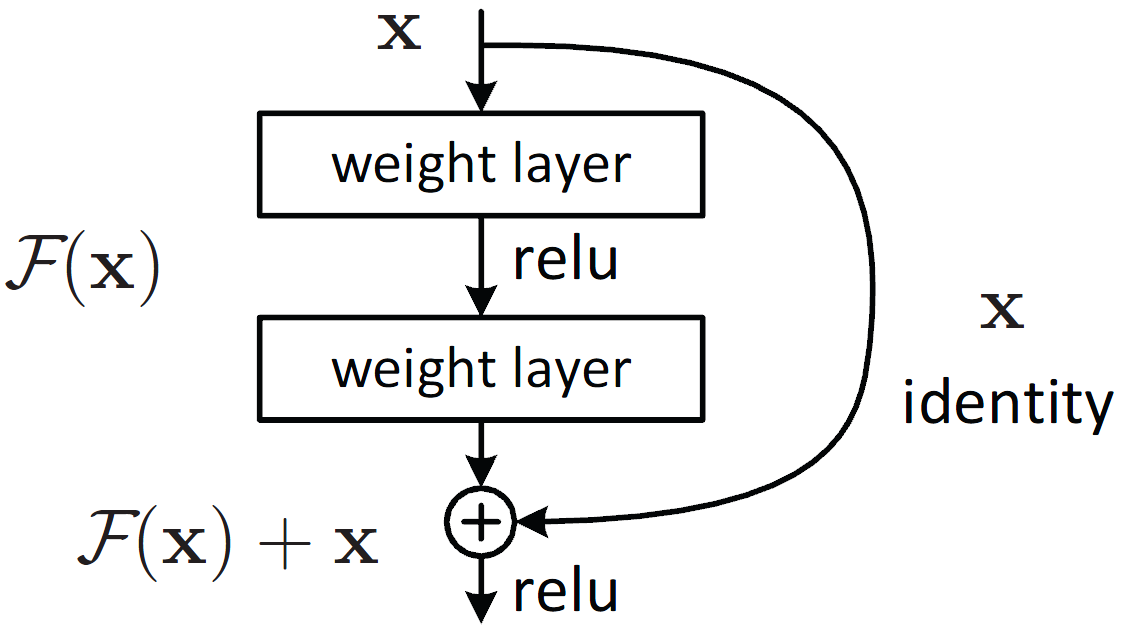
\includegraphics[width=0.44\textwidth]{../img/residual_block.png}
	\caption{Residual block (\cite{He2016}).}
	\label{fig:residual_block}
\end{figure}

The identity mapping helps the gradient propagate more effectively through the neural network, even in deep architectures. It also provides the network with the ability to skip the transformation $\mathcal{F}(x)$ entirely, in cases where the identity mapping is optimal. This also allows the network to learn residuals as small adjustments to the identity function, rather than requiring the network to learn a complete transformation from scratch.

Now, we can define the plain network as described in \cite{He2016}, which serves as the basis for ResNet. The plain network was inspired by VGG nets, which were the state-of-the-art architecture at the time of publication (see \cite{Simonyan2014}). The network starts with a convolutional layer with kernel size $7 \times 7$, continuing with many convolutional layers with kernel size $3 \times 3$. Two design rules are followed. When performing convolution with a stride of 1, the number of kernels matches the number of input channels. However, when using a stride of 2, the number of kernels doubles to preserve the complexity. The network ends with a global average pooling layer and a fully-connected layer. The VGG type network (VGG-19) and the plain network are shown in Figure~\ref{fig:resnet} (left and middle, respectively).

A Residual Neural Network is constructed from the plain network by introducing shortcuts, every two layers, as shown in Figure~\ref{fig:resnet} (right), where solid lines represent the use of Equation~(\ref{residual_block_identity}), and dotted lines represent the use of Equation~(\ref{residual_block_projection}).

There are different variants of ResNet models, distinguished by the number of layers, which affect their capacity and performance. The most commonly used variants are ResNet18, ResNet34, ResNet50, ResNet101, and ResNet152, where the number indicates the total number of layers.

\begin{figure}[h!]
	\centering
	\includegraphics[width=0.6\textwidth]{../img/resnet.png}
	\caption{Example of network architecture (\cite{He2016}). Left: VGG-19 model as a reference. Middle: a plain network with 34 layers. Right: residual network with 34 layers (ResNet34).}
	\label{fig:resnet}
\end{figure}
\chapter{Experimental Evaluation of Rényi-based Knowledge Distillation}

This chapter is dedicated to applying the modified knowledge distillation process, in which Rényi divergence is used in place of the traditional Kullback–Leibler (KL) divergence. The experimental evaluation is conducted using the ResNet architecture on the CIFAR-100 dataset.

In the first experiment, we compare the performance of standard knowledge distillation with that of the Rényi-based approach. The second experiment extends this comparison by evaluating the results of two newly formulated Rényi-based knowledge distillation setups against those from the previous experiment.

\section{Dataset}

The dataset used for our experiments is CIFAR-100, which was introduced in \cite{Krizhevsky2009} as a subset of a larger dataset created by \cite{TorralbaFergusFreeman2008}. It consists of 60,000 labeled color images across 100 classes, with 600 images per class. There are 50,000 images in the training set and 10,000 images in the test set. All images are downscaled to $32 \times 32$ pixels. The 100 classes in the dataset are grouped into 20 so-called superclasses.

As an example we select two superclasses called \textit{large omnivores and herbivores} and \textit{household furniture}. The first contains classes \textit{camel}, \textit{cattle}, \textit{elephant}, \textit{chimpanzee} and \textit{kangaroo}, while the second one contains classes \textit{bed}, \textit{couch}, \textit{chair}, \textit{table} and \textit{wardrobe}. Clearly, the classes within the same superclass are much more similar than those across superclasses, often sharing the same textures, shapes, or color patterns as can be seen in Figure~\ref{fig:cifar100}.

\begin{figure}[h!]
	\centering
	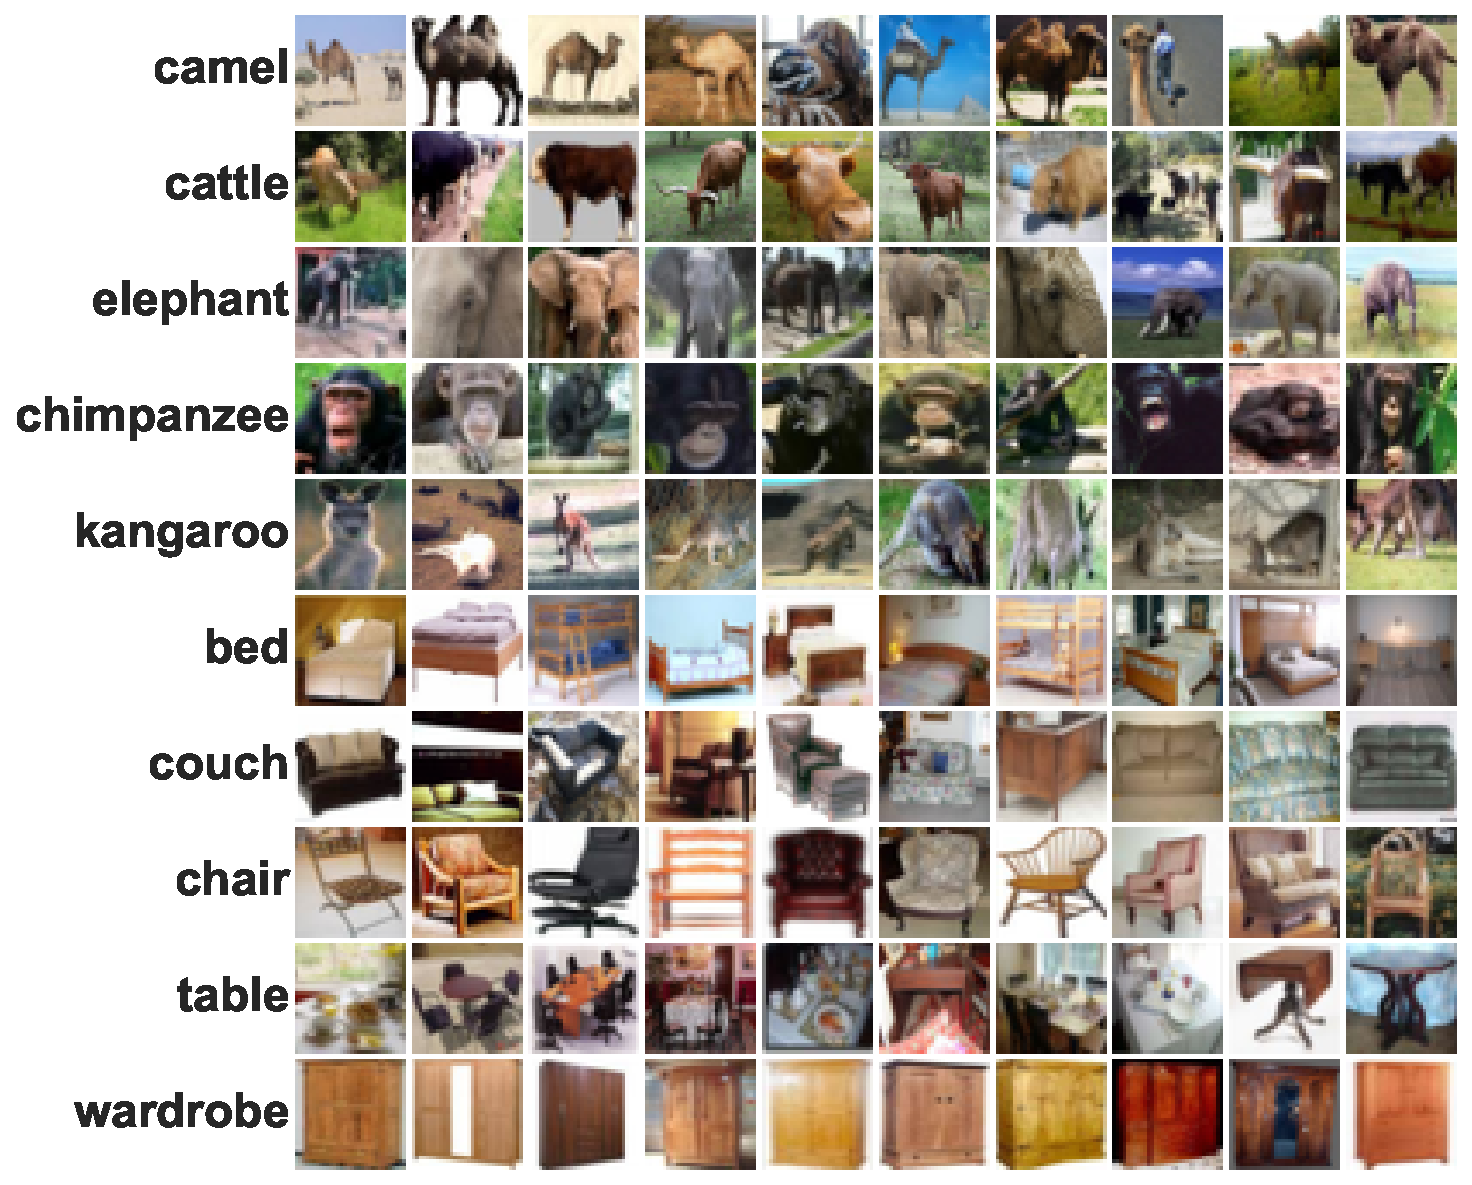
\includegraphics[width=0.57\textwidth]{../img/cifar100_grid.pdf}
	\caption{Visualization of 10 randomly selected images from each of the 5 classes within the superclasses \textit{large omnivores and herbivores} (top) and \textit{household furniture} (bottom) from the CIFAR-100 dataset.}
	\label{fig:cifar100}
\end{figure}

\section{Experiment 1}

In this first experiment, we evaluate the performance of Rényi-based knowledge distillation, which introduces a hyperparameter $\alpha \in [0, \infty]$. When $\alpha = 1$, the loss function is equivalent to that of standard knowledge distillation, providing a natural baseline for comparison.

For the experimental setup, we chose ResNet152 as the architecture for the teacher model and ResNet18 for the student model. We thus chose the teacher model to be much larger ($11.3 \times 10^9$ parameters) compared to the student model ($1.8 \times 10^9$ parameters) to exaggerate the performance difference between the models, thereby increasing the potential for improvement during knowledge distillation and allowing us to more reliably evaluate the impact of the various modifications introduced to the student model testing.

Training was performed using the Python programming language and the Timm library (\cite{Wightman2019}), which provides various advanced methods for optimization, regularization, and data augmentation, along with many pre-built models, including various ResNet architectures. However, it does not include support for knowledge distillation and Rényi loss. Thus, we needed to modify parts of the code to support both standard and Rényi-based knowledge distillation.

Given the large number of hyperparameters to tune in the Timm library, we decided to adopt a configuration strategy inspired by \cite{AbbasLee2021}, which aimed to optimize the performance of ResNet models on the CIFAR-100 dataset. The hyperparameters used are summarized in Table~\ref{tab:hyperparams} below. A notable modification we made was increasing the batch size and learning rate by a factor of four, which, as shown in \cite{Goyal2017}, does not substantially affect overall performance. Our motivation for this change was to speed up the training process. Additionally, we did not apply dropout to the fully connected layer and extended the number of epochs by 20, both of which are minor changes that had no significant impact on performance. The motivation behind these changes was to stabilize performance fluctuations between successive epochs at the end of the training.

\begin{table}[h]
	\centering
	\begin{tabular}{lc}
		\toprule
		\textbf{Hyperparameter}     & \textbf{Value} \\ \midrule
		Optimizer                    & SGD            \\
		Learning rate\tablefootnote{Learning rate decay was applied during training as a standard machine learning procedure.} & 0.08 \\
		Momentum                     & 0.9            \\
		Weight decay                 & 0.0005       \\
		Epochs                       & 220            \\
		Batch size                   & 512            \\
		Activation function          & ReLU           \\
		\bottomrule
	\end{tabular}
	\caption{Training hyperparameters used for the experiment inspired by \cite{AbbasLee2021}.}
	\label{tab:hyperparams}
\end{table}

We also introduce data augmentation, which refers to modifications applied to the dataset to improve the model’s generalization ability, such as rescaling, cropping, and flipping images, as suggested by \cite{Wightman2021}.

First, using the training setup described above, we train both the ResNet152 and ResNet18 models on the train set without applying knowledge distillation, that is, using vanilla training, as described in the first chapter. The first model is the teacher model for knowledge distillation, while the second model, referred to as the vanilla model, shares the same architecture as the student model but is trained independently, without knowledge distillation. This model serves as our benchmark against which the results of knowledge distillation are compared.

In Figure~\ref{fig:teacher_vanilla_model}, we observe the performance of the models, measured by the test accuracy on the CIFAR-100 dataset. As expected, the teacher model performs better, achieving a final accuracy of 68.06\%, compared to the vanilla model, which ended training with an accuracy of 62.61\%. Since the test set contains 10,000 images, the difference between the two models corresponds to 545 images being correctly/incorrectly classified. Looking closely, we observe that the two models performed similarly during the first 50 epochs. Afterward, the teacher model began improving at a faster rate than the student.

\begin{figure}[h!]
	\centering
	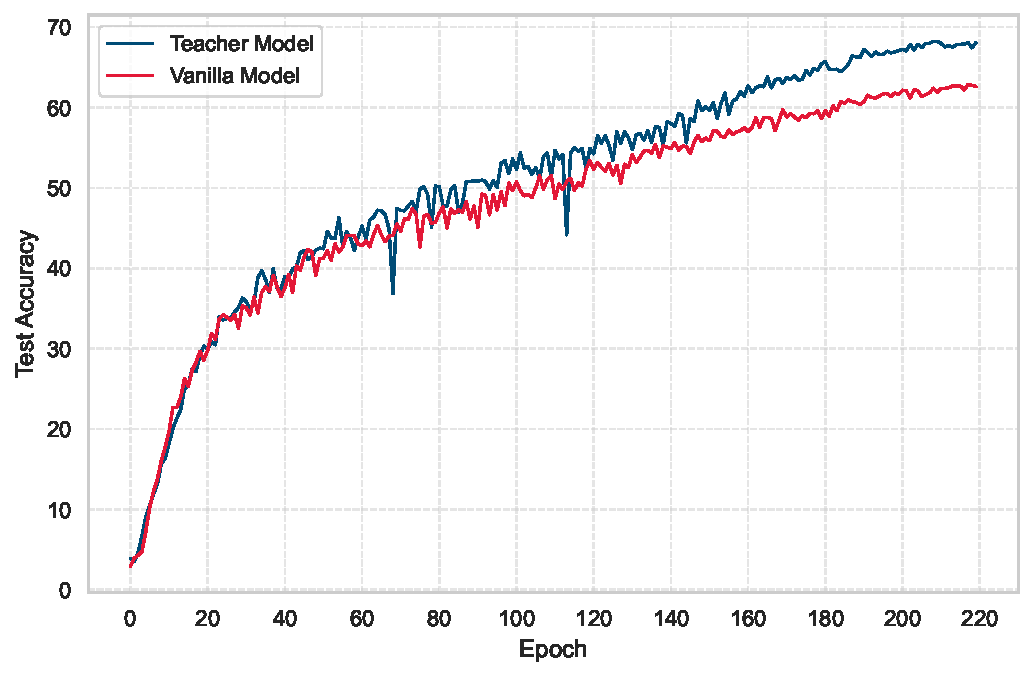
\includegraphics[width=0.7\textwidth]{../img/teacher_vanilla_model.pdf}
	\caption{Test accuracy over 220 epochs for the teacher and vanilla models.}
	\label{fig:teacher_vanilla_model}
\end{figure}

Now, we turn our attention to knowledge distillation, which requires additional three hyperparameters, as shown in Equations~(\ref{Rényi Knowledge Distillation}) and (\ref{Rényi loss}): $\alpha$, $\beta$, and the temperature $T$. We do not aim to optimize the hyperparameters $\beta$ and $T$, therefore, we adopt a commonly used choice discussed previously: $\beta = 0.9$ and $T = 4$.

The hyperparameter $\alpha$ is the primary focus of this experiment. We trained student model for each choice of $\alpha$ in Table~\ref{tab:exp1_res} with Rényi-based knowledge distillation with 10 different seeds. We report the average test accuracy and accuracy improvement over the vanilla model. Recall that $\alpha=1$ corresponds to the standard knowledge distillation. Unaggregated results are further shown in Figure~\ref{fig:exp1_box_219} in the form of boxplots.

\begin{table}[h]
	\centering
	\begin{tabular}{lcc}
		\toprule
		& \textbf{Average} & \textbf{Improvement over} \\
		$\boldsymbol{\alpha}$ & \textbf{Accuracy} & \textbf{Vanilla Model} \\ \midrule
		0.05 & 64.107 & 1.497 \\
		0.1 & 63.953 & 1.343\\
		0.25 & 64.063 & 1.453\\
		0.5 & 64.067 & 1.457\\
		0.625 & 64.072 & 1.462\\
		0.75 & 64.062 & 1.452\\
		0.875 & 64.086 & 1.476\\
		1 & 64.200 & 1.590 \\
		\bf{1.25} & \bf{64.277} & \bf{1.667} \\
		1.5 & 64.027 & 1.417 \\
		2 & 64.218 & 1.608\\
		3.5 & 64.242 & 1.632\\
		5 & 63.946 & 1.336\\
		7.5 & 63.757 & 1.147\\
		10 & 63.560 & 0.950\\
		12.5 & 63.387 & 0.777\\
		\bottomrule
	\end{tabular}
	\caption{Experiment 1 results showing average test accuracy and improvement over the vanilla model for various values of $\alpha$. The best result is highlighted in bold.}
	\label{tab:exp1_res}
\end{table}

We begin with the standard knowledge distillation, i.e., $\alpha = 1$, the average accuracy is 64.200\%, which is 1.590\% better than the vanilla model and looking at the boxplot in Figure 3.3 we see that the minimal improvement is around 1.2\% which confirms the well-established understanding that the standard knowledge distillation improves the student model performance. This gap means that, on average, 159 more test images are correctly classified.

\begin{figure}[h!]
	\centering
	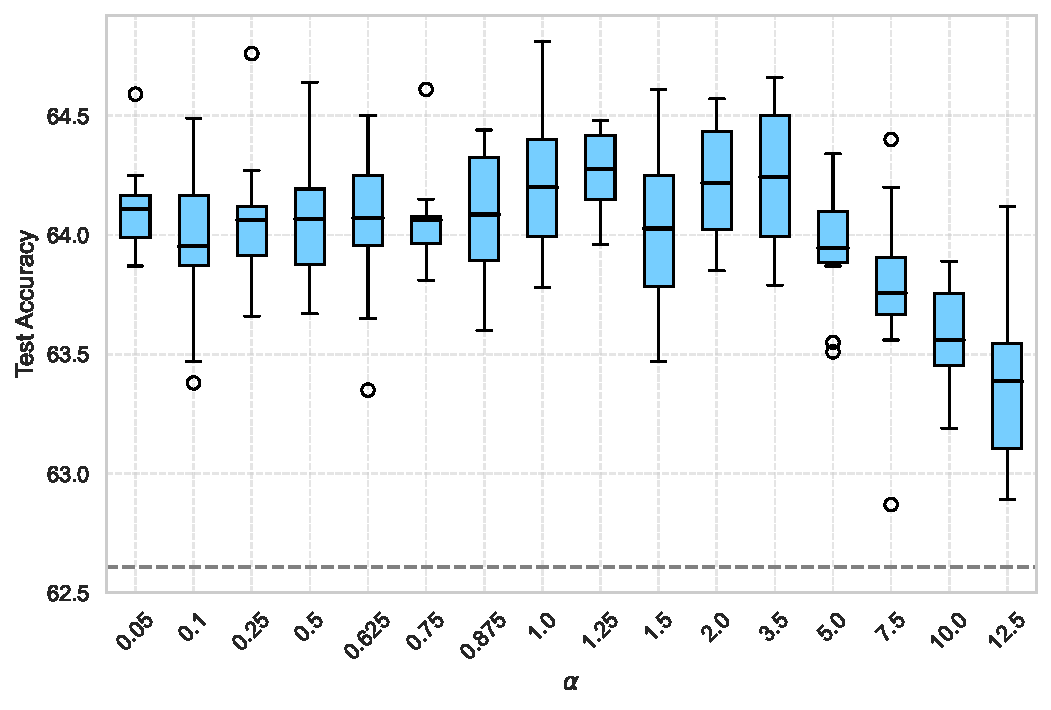
\includegraphics[width=0.7\textwidth]{../img/exp1_box_220.pdf}
	\caption{Boxplots of the performance of fully-trained models from Experiment 1, with average values indicated by black lines and the performance of the vanilla model represented by a dashed gray line.}
	\label{fig:exp1_box_219}
\end{figure}

Concentrating on the averages (and thus neglecting standard deviation), the models with values $\alpha$ between 1 and 3.5 perform the best. For $\alpha \geq 5$ the performance deteriorates, while still outperforming the vanilla model.

The most promising models are those with $\alpha = 1.25,\; 2,\; 3.5$. All of them outperform the standard knowledge distillation model, with $\alpha = 1.25$ achieving the best average accuracy of 64.277\%, which is 0.077\% higher than the accuracy for $\alpha = 1$. This further reduces the performance gap between the vanilla and teacher models by an additional 1.4\%, bringing the total reduction to 30.5\%.

These results, however, are not sufficient to conclude that choosing $\alpha = 1.25$ yields a statistically significant improvement over $\alpha = 1$. Nevertheless, we cannot rule out the possibility that this is indeed the case. More extensive testing is needed to draw definitive conclusions regarding this possibility.

In contrast, more promising results from a different perspective can be found in Figure~\ref{fig:exp1_box_10}, which depicts the performance of the models after only 10 epochs out of 220. It can be observed that only the student models corresponding to $\alpha$ values of 3.5, 5, or 7.5 significantly outperform the vanilla model. While lower values of $\alpha$ lead to deteriorating performance, both $\alpha = 1$ and $\alpha = 1.25$ trail behind the best-performing model with $\alpha = 5$.

\begin{figure}[h!]
	\centering
	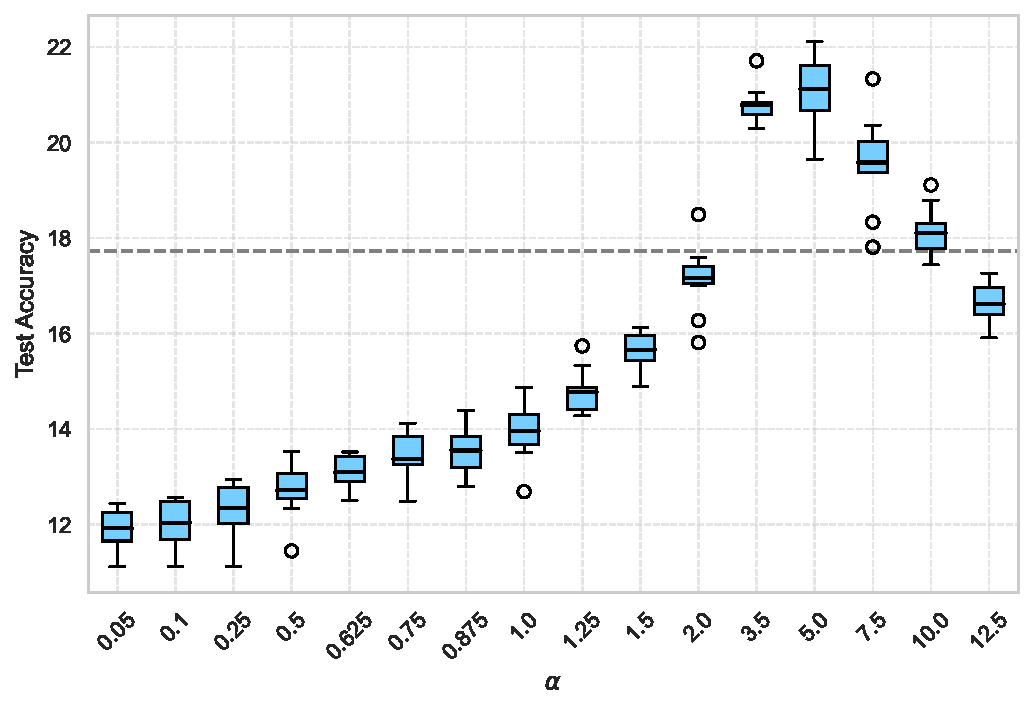
\includegraphics[width=0.7\textwidth]{../img/exp1_box_10.pdf}
	\caption{Boxplots of the performance of models from Experiment 1 after 10 epochs, with average values indicated by black lines and the performance of the vanilla model represented by a dashed gray line.}
	\label{fig:exp1_box_10}
\end{figure}

These results are not limited to the tenth epoch, as shown in Figure~\ref{fig:exp1_line_and_diff_plot}, which compares the aforementioned models, similar trends are observed across many early epochs of the training. This suggests that during training, higher values of $\alpha$ enable the student model to learn faster in the first few epochs.

The figure shows that the student model with $\alpha = 5$ outperforms all others in the early stages of training, with its advantage over the standard knowledge distillation model peaking around epochs 10 to 20 at approximately 5\% higher accuracy. The advantage shirks until epoch 70, where there is no longer any noticeable difference in performance. A similar pattern is observed for $\alpha = 1.25$, where the accuracy difference is smaller (around 1\%) but remains stable between epochs 10 and 50.

\begin{figure}[h!]
	\centering
	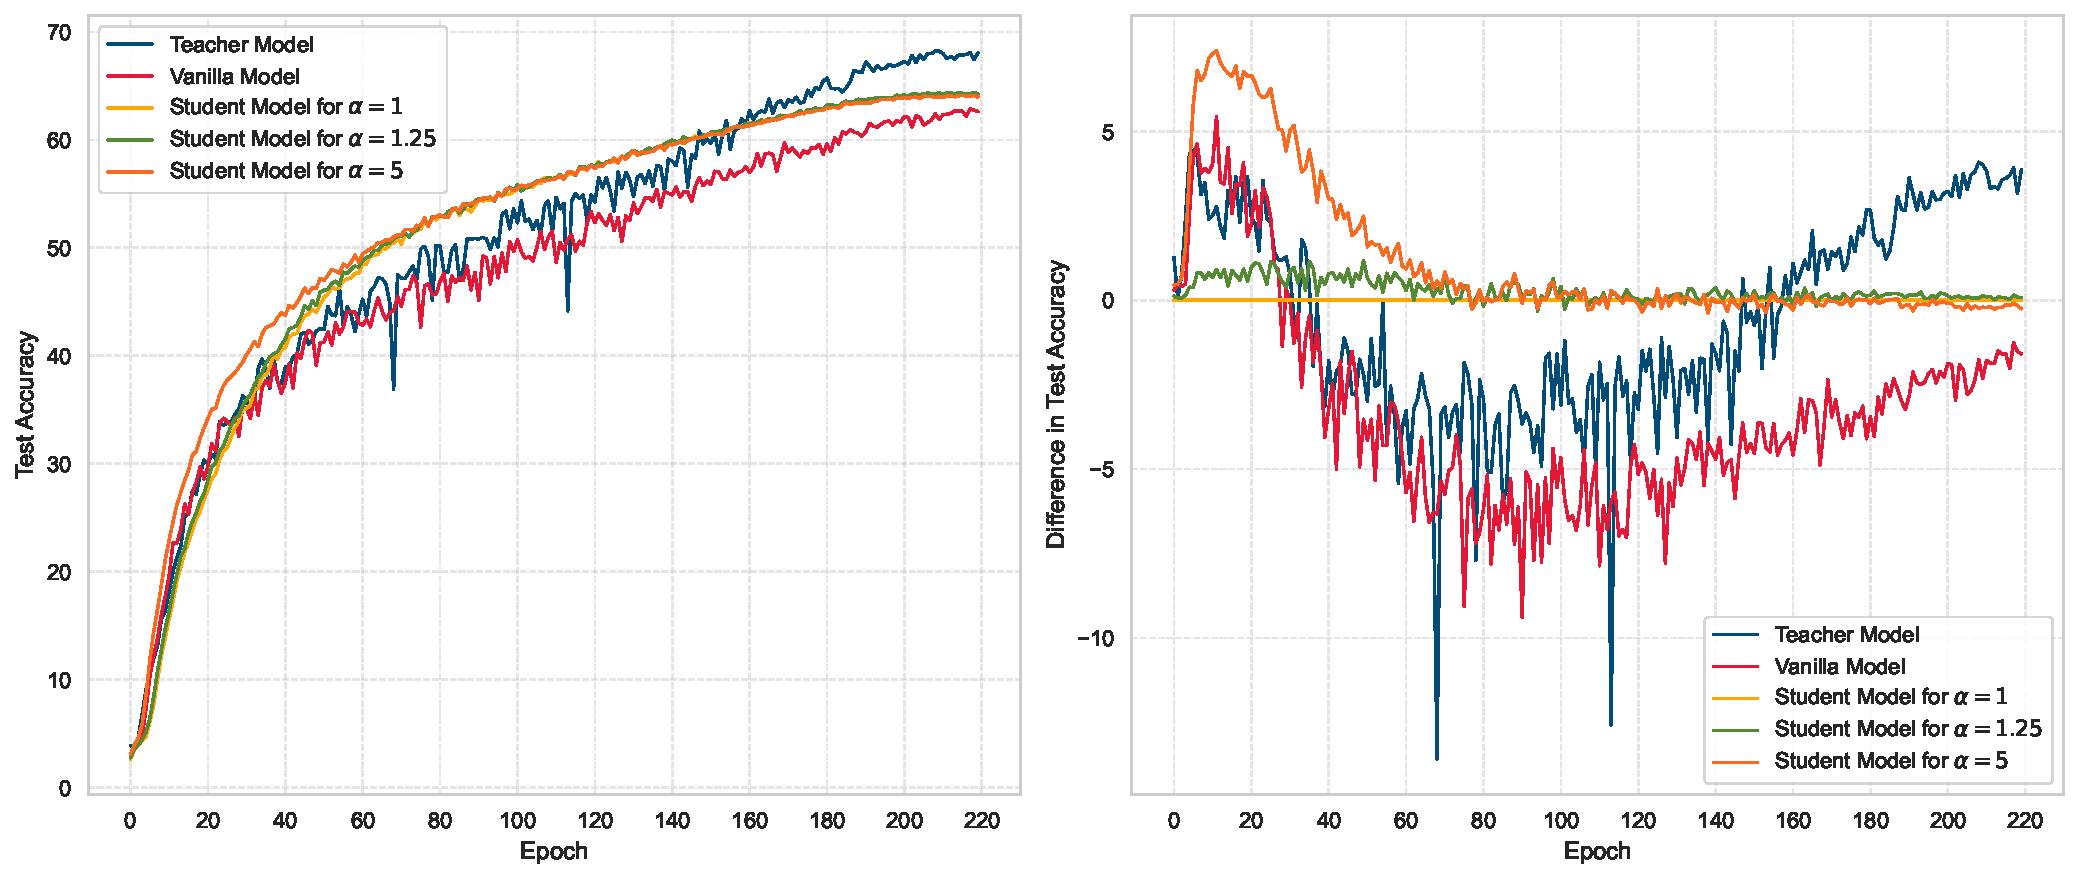
\includegraphics[width=1\textwidth]{../img/exp1_line_and_diff_plot.pdf}
	\caption{Comparison of the models. Left: Validation accuracy over 220 epochs for the teacher, vanilla, and selected student models. Right: Difference in accuracy compared to the student model with $\alpha=1$ over 220 epochs (Student models show averages over 10 iterations).}
	\label{fig:exp1_line_and_diff_plot}
\end{figure}

The performance difference between both the teacher and the vanilla models compared to the standard knowledge distillation model evolves over time. In the early stages, the vanilla-trained models slightly outperform the student model for $\alpha=1$, but around epoch 20, their performance begins to decline, and by epoch 90, they fall behind all student models by approximately 4\% in accuracy. After that point, both the teacher and the vanilla model continue to improve, albeit at different rates. While the teacher ultimately outperforms the student models, the vanilla model consistently remains behind all of them.

\section{Experiment 2}

This experiment extends the previous experiment by introducing two alternative formulations of the Rényi loss function from Equation~(\ref{Rényi loss}) and conducting tests similar to those in Experiment 1.

This has been motivated by the result of the preliminary testing. There we monitored various internal metrics of the student models, such as gradient behavior, to ensure that training with the Rényi loss function is numerically stable and exhibited well-conditioned optimization behavior. One of the monitored metrics is defined as

\begin{equation*}
	\kappa = \max_{(x,y) \in \mathcal{B},\, j} \left| \frac{v_j\, z_j}{T^2} \right|,
\end{equation*}
where $\mathcal{B}$ denotes the final batch of a given epoch, $v_j$ and $z_j$ the logits produced by the teacher and student models respectively, and $T$, the temperature hyperparameter, is fixed at 4.

This metric is connected to the assumption stated in Equation~\ref{assumption negligible}, particularly regarding the negligibility of the term $\frac{v_j z_j}{T^2}$. The assumption was used in deriving the result that the gradient of the Rényi loss function decreases proportionally to $\frac{\alpha}{T^2}$. This insight motivated the formulation of the Rényi loss function as shown in Equation~(\ref{Rényi loss}), which explicitly includes the scaling term $\frac{T^2}{\alpha}$.

Figure~\ref{fig:xy_T2} depicts the evolution of $\kappa$ during training, showing a steady increase over time, ultimately reaching approximately 5.5. Thus, it is evident that the assumption of negligibility of $\frac{v_j z_j}{T^2}$ does not generally hold.

\begin{figure}[h!]
	\centering
	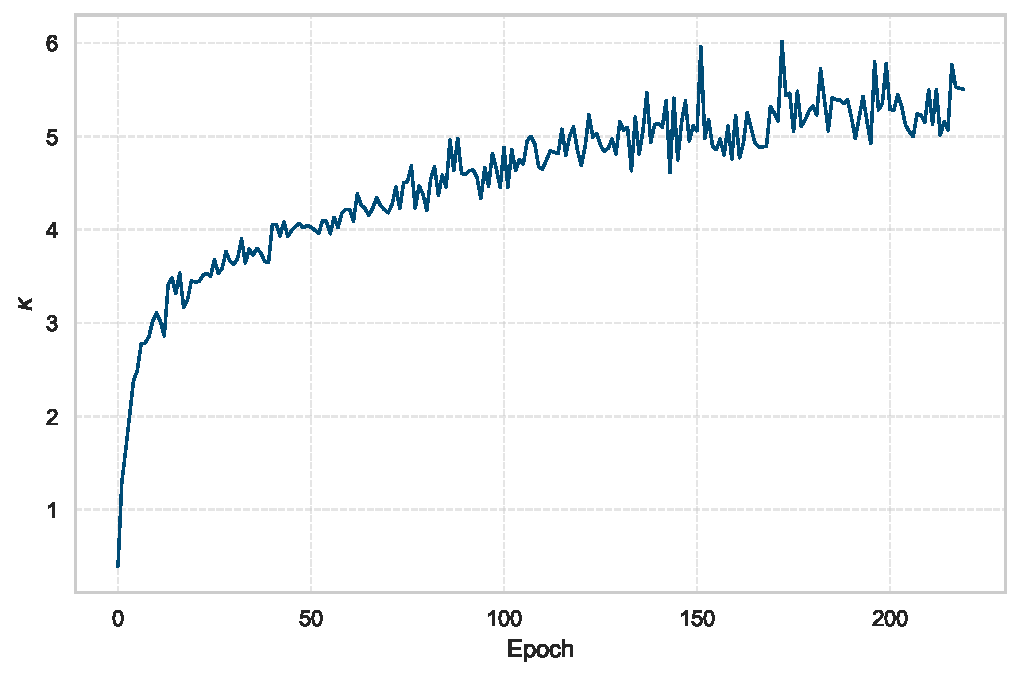
\includegraphics[width=0.7\textwidth]{../img/xy_T2.pdf}
	\caption{Average value of $\kappa$ during testing across all models, computed by averaging over various values of $\alpha$, with $T=4$, as observed in the preliminary testing.}
	\label{fig:xy_T2}
\end{figure}

This behavior arises from the temperature not being sufficiently high. However, as noted in the case of standard knowledge distillation by \cite{HintonVinyalsDean2015}, this may not be a critical issue. In any case, this prompted us to examine how the gradient of the Rényi loss function with respect to the logits of the student model behaves as a function of the hyperparameter $\alpha$.

In the previous experiment, we observed that the performance of student models corresponding to different values of $\alpha$ diverges most significantly at the beginning of the training. Thus, we focus on the initial phase of the training, using an untrained ResNet18 model as the student and a fully-trained ResNet101 model on CIFAR-100 as the teacher. To calculate the gradient we use Equation~(\ref{Rényi gradient}).

We calculate the gradients for 1,000 images from the training set, resulting in 100,000 different values, as each image produces 100 values corresponding to the 100 classes. Both the teacher and the student output a prediction by selecting the class with the highest logit among the 100 possible classes. We use this prediction to label the gradients. We assign a label of 11 to a value if the corresponding class is predicted by both models. A label of 10 is assigned if only the teacher predicts the class, 1 if only the student model does, and 0 if neither.

We expect the vast majority of the values to be labeled as 0, since each model predicts only one class out of 100. Since the untrained student model is essentially a random number generator, it always predicts a random class. As a result, only a small number of values will be labeled as 11, that is predicted by both models simultaneously.

The motivation for introducing these labels is that, for both fully trained models, classes 1, 10, and 11 correspond to high logit values produced by the student, the teacher, and both models, respectively. Without separating them from class 0, these values would appear as outliers. This is undesirable, as the behavior of these values provides valuable insight into the training process.

Figure~\ref{fig:gradients_boxplot_adjusted} shows the gradients in form of boxplots for different values of $\alpha$, grouped according to their assigned labels. We observe, that the behavior of classes 0 and 1 are similar, the same is true for classes 10 and 11. This again results from the fact that the student model is untrained, so the largest logit is expected to have a similar magnitude to the other logits. This would not be true for trained student model.

\begin{figure}[h!]
	\centering
	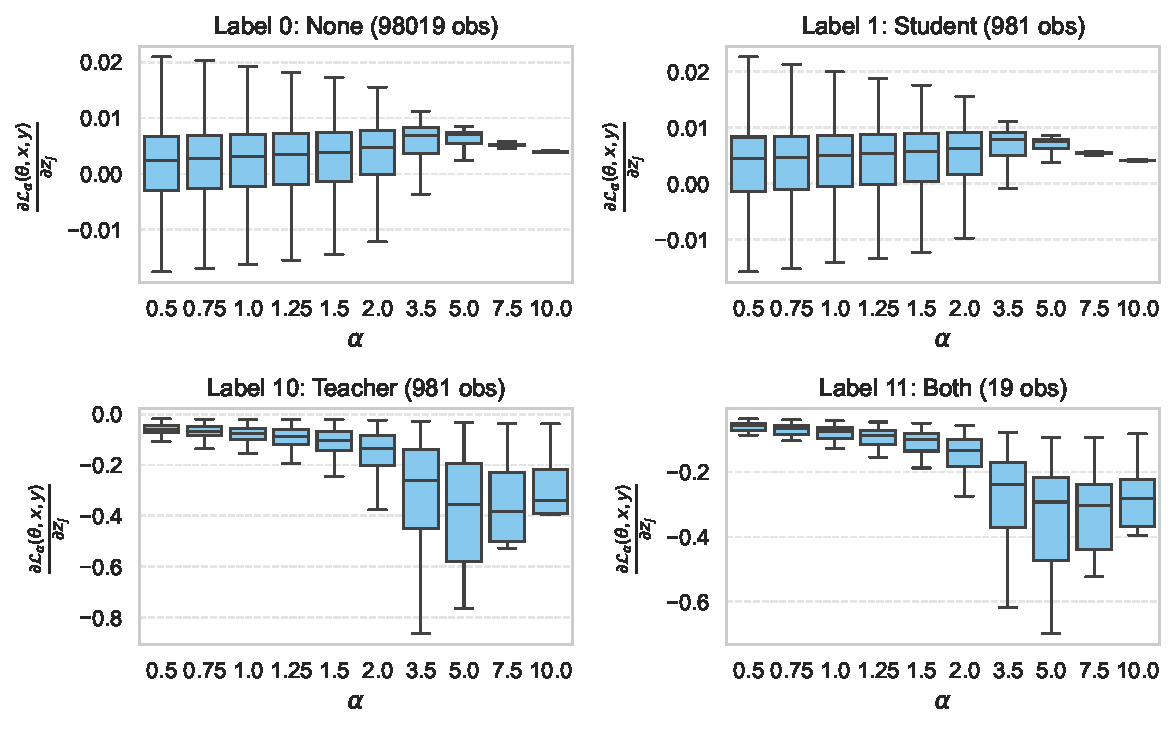
\includegraphics[width=0.7\textwidth]{../img/gradients_boxplot_adjusted.pdf}
	\caption{Boxplots of the gradient values of the Rényi loss with respect to the student model logits, across various values of $\alpha$, grouped by label, for $T=4$.}
	\label{fig:gradients_boxplot_adjusted}
\end{figure}

The differences in gradients for varying values of $\alpha$ for labels 1, 10 and 11 are desirable, as they represent one of the key factors that cause the training process to differ across values of $\alpha$. What may be considered undesirable, however, is the variation in the medians for label 0, as it suggests an inconsistent learning rate across different settings, especially for larger values of $\alpha$. Additionally, we observe that the variance decreases, which might be one of the factors contributing to the lower performance observed for larger values of $\alpha$ in Experiment 1.

There are two approaches we might consider. Firstly, since the conditions required to simplify the derivative of the Rényi divergence are quite restrictive, we might choose not to use the scaling term $\frac{T^2}{\alpha}$. Instead, we consider a solution which has been already used by \cite{HintonVinyalsDean2015} for the case of the standard knowledge distillation and might be a viable in our case. There, we simply replace the KL divergence with the Rényi divergence in Equation~(\ref{KL loss}), resulting in the following unscaled Rényi loss function

\begin{equation}
	\mathcal{L}_{\alpha,\text{unscaled}}(\theta,x,y) = T^2 D_\alpha(P^T \| Q^T).
	\label{modified_RL_noadj}
\end{equation}

Alternatively, we may aim to find a scaling function $\phi(\alpha,T)$ that keeps the median of the gradients for label 0 constant across varying values of $\alpha$, thereby normalizing them, resulting in the normalized Rényi loss function

\begin{equation}
	\mathcal{L}_{\alpha,\text{norm}}(\theta,x,y) = \phi(\alpha,T) D_\alpha(P^T \| Q^T).
	\label{modified_RL_sigmoid}
\end{equation} 

\paragraph{Unscaled loss} In Figure~\ref{fig:gradients_boxplot_noadj} and, we present a graphs analogous to Figure~\ref{fig:gradients_boxplot_adjusted}, calculated using the unscaled loss function given in Equation~(\ref{modified_RL_noadj}). There, we observe that the median of the gradients for label 0 varies even more across different values of $\alpha$, compared to the previous approach. This implies that changing $\alpha$ indirectly affects the effective learning rate. One of the implications is the possibility of better performance of the student model during the initial epochs. Also note that the variance differs, peaking at $\alpha = 2$, while becoming particularly small for larger values of $\alpha$.

\begin{figure}[h!]
	\centering
	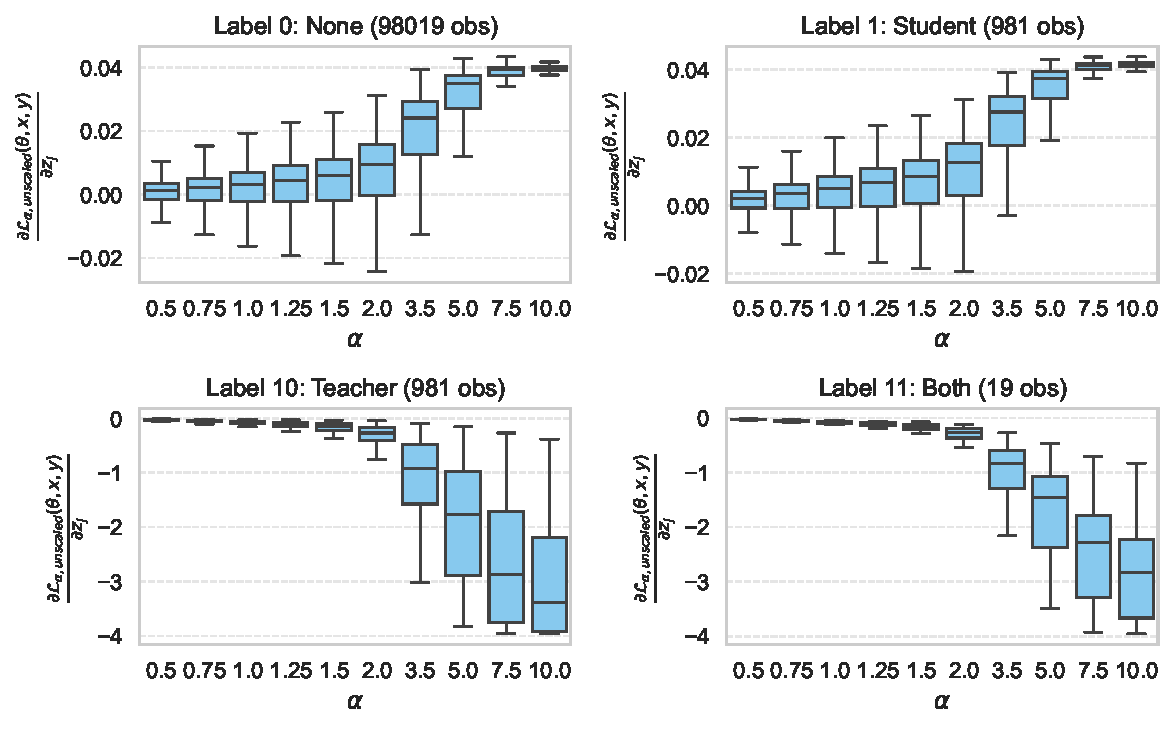
\includegraphics[width=0.7\textwidth]{../img/gradients_boxplot_noadj.pdf}
	\caption{Boxplots of the gradient values of the unscaled Rényi loss from Equation~(\ref{modified_RL_noadj}) with respect to the student model logits, across various values of $\alpha$, grouped by label, for $T=4$.}
	\label{fig:gradients_boxplot_noadj}
\end{figure}

For the second approach, we need to estimate the function $\phi(\alpha,T)$. We require that $\phi(1,T)=T^2$, as this ensures the training process is equivalent to standard knowledge distillation, i.e., when $\alpha=1$. In our case, we focus exclusively on $T=4$, as this is the temperature used in all experiments.

We first estimate the behavior of the gradients when setting $\phi(\alpha,T)=T^2$ for all values of $\alpha$, which reduces the normalized loss function from Equation~(\ref{modified_RL_sigmoid}) to the form given in Equation~(\ref{modified_RL_noadj}). Thus, we can use the results from Figure~\ref{fig:gradients_boxplot_noadj} as a reference while computing additional values for other settings of $\alpha$. These results can be seen in Figure~\ref{fig:sigmoid_approx}. We immediately recognize the shape of the curve as resembling a sigmoid-like function. Therefore, we fit a sigmoid function to the data, denoted as $\sigma(\alpha)$ which, upon fitting, is given by the following expression

\begin{equation*}
	\hat{\sigma}(\alpha) = \frac{0.0416}{1 + e^{-(0.9968\, \alpha - 2.9970)}} - 0.0018.
\end{equation*}
The relationship between the function $\sigma(\alpha)$ and $\phi(\alpha,4)$ is as follows

\begin{equation*}
	\phi(\alpha,4) = \frac{\sigma(1)}{\sigma(\alpha)} 4^2,
\end{equation*}
since $\sigma(\alpha)$ approximates the median of the gradients labeled as 0, dividing the loss function by $\sigma(\alpha)$ results in a constant median of these gradients. Additionally, $\phi(1,4)=4^2$, as required.

\begin{figure}[h!]
	\centering
	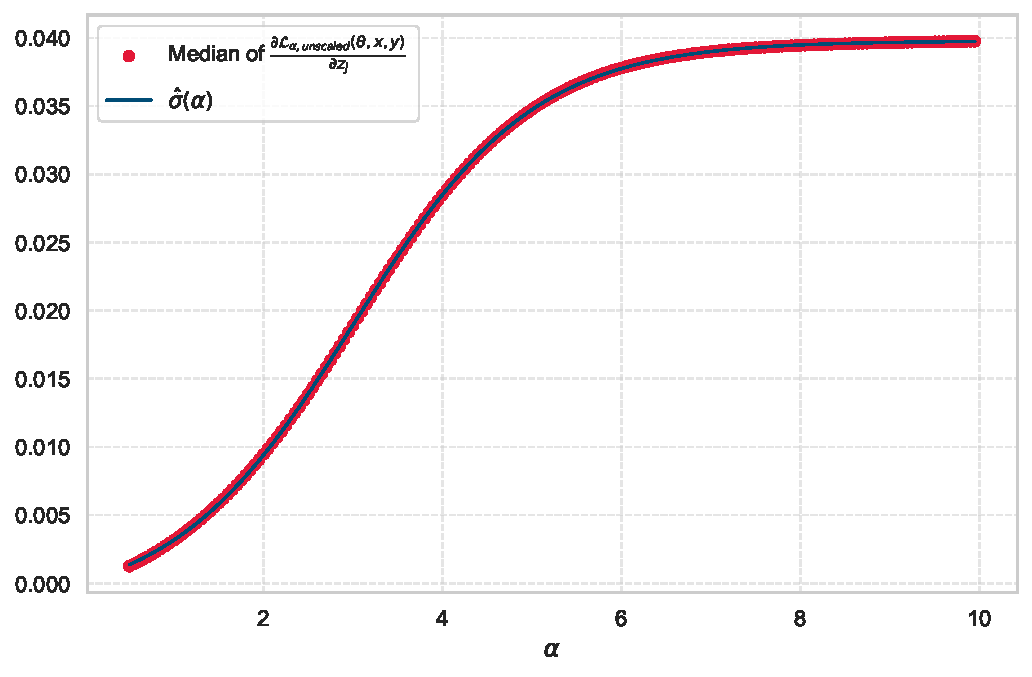
\includegraphics[width=0.7\textwidth]{../img/sigmoid_approx.pdf}
	\caption{Medians of gradient values for label 0, computed using the unscaled Rényi loss from Equation~(\ref{modified_RL_noadj}) with respect to the student model logits, across various values of $\alpha$, along with the function $\hat{\sigma}(\alpha)$ estimated from this data}
	\label{fig:sigmoid_approx}
\end{figure} 

Using this approach with the fitted $\hat{\phi}(\alpha,4)$, we compute the gradients analogously to the previous figures, resulting in Figure~\ref{fig:gradients_boxplot_sigmoid}. As observed, the medians of the gradients for label 0 remain constant, as intended. The variance diminishes with increasing $\alpha$, similarly to the case of the original Rényi-based knowledge distillation.

\begin{figure}[h!]
	\centering
	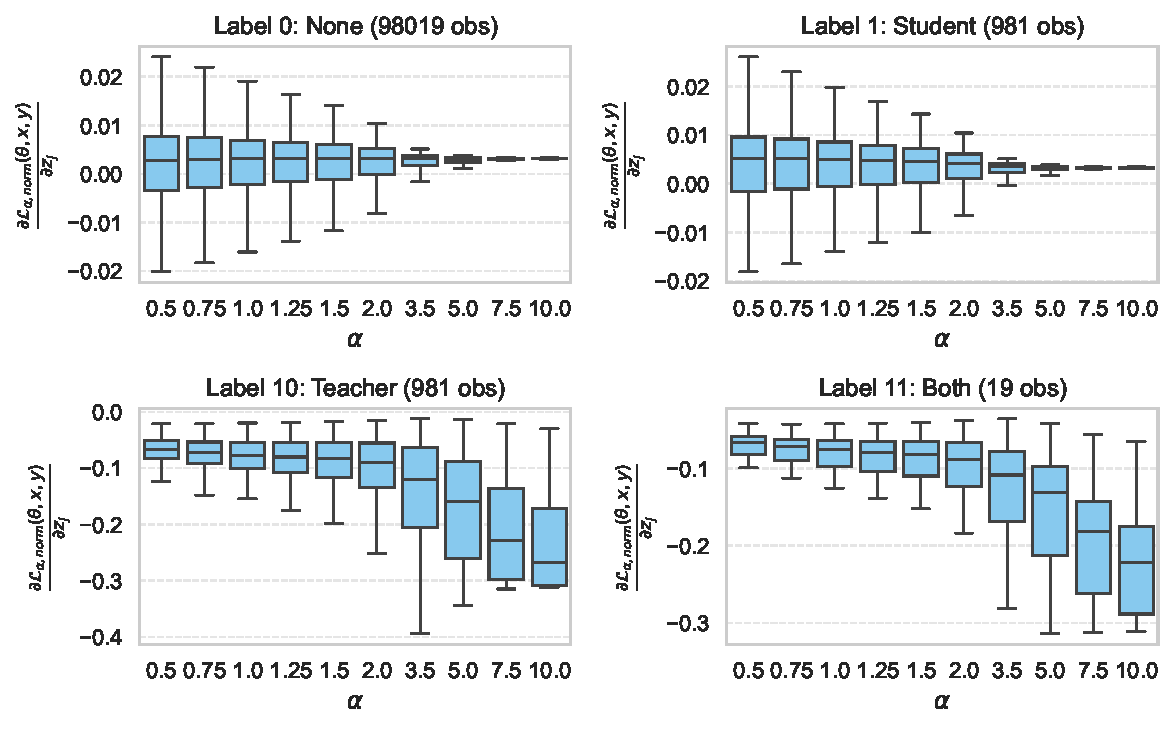
\includegraphics[width=0.7\textwidth]{../img/gradients_boxplot_sigmoid.pdf}
	\caption{Boxplots of the gradient values of the normalized Rényi loss from Equation~(\ref{modified_RL_sigmoid}) with respect to the student model logits, across various values of $\alpha$, grouped by label, for $T=4$.}
	\label{fig:gradients_boxplot_sigmoid}
\end{figure}

Following the introduction of the two approaches and a brief analysis of their gradients, we aim to directly compare them to the results of Experiment 1 using the CIFAR-100 dataset. We now train student model for each choice of $\alpha$ from the Table~\ref{tab:exp2_res} with modified Rényi knowledge distillation with 10 different seeds. As before, we report the average test accuracy, with the accuracy improvement over the vanilla model shown as a superscript.

\begin{table}[h]
	\centering
	\begin{tabular}{lccc}
		\toprule
		$\boldsymbol{\alpha}$ & $\bf{Original}$ & $\bf{Unscaled}$ & $\bf{Normalized}$ \\ \midrule
		0.5 & $64.067^{1.457}$ & $63.855^{1.245}$ & $64.367^{1.757}$ \\
		0.625 & $64.072^{1.462}$ & $64.099^{1.489}$ & $64.216^{1.606}$ \\
		0.75 & $64.062^{1.452}$ & $63.961^{1.351}$ & $64.295^{1.685}$ \\
		0.875 & $64.086^{1.476}$ & $64.206^{1.596}$ & $64.297^{1.687}$ \\
		1.0 & $64.200^{1.590}$ & $64.281^{1.671}$ & $64.311^{1.701}$ \\
		1.25 & $\bf{64.277^{1.667}}$ & $\bf{64.499^{1.889}}$ & $64.196^{1.586}$ \\
		1.5 & $64.027^{1.417}$ & $64.370^{1.760}$ & $\bf{64.373^{1.763}}$ \\
		2.0 & $64.218^{1.608}$ & $64.480^{1.870}$ & $64.343^{1.733}$ \\
		3.5 & $64.242^{1.632}$ & $64.130^{1.520}$ & $64.042^{1.432}$ \\
		5.0 & $63.946^{1.336}$ & $64.246^{1.636}$ & $64.034^{1.424}$ \\
		7.5 & $63.757^{1.147}$ & $63.802^{1.192}$ & $63.868^{1.258}$ \\
		\bottomrule
	\end{tabular}
	\caption{Results of Experiment 2 showing the average test accuracy for various values of $\alpha$, with the improvement over the vanilla model in superscript. The best result for each loss function is highlighted in bold.}
	\label{tab:exp2_res}
\end{table}

First, we note that for $\alpha=1$, all approaches are equivalent. That being said, the results for different loss functions shown in the table differ noticeably, suggesting that the average accuracy of the model over ten seeds can fluctuate by more than 0.1\%. Therefore, any difference within 0.1\% should not be considered statistically significant.

The best performance was achieved with $\alpha=1.25$ and the unscaled loss function, achieving an average accuracy of 64.449\%, which is 1.889\% higher than the vanilla model and 0.222\% higher than the best model from Experiment 1. Furthermore, it reduces the gap between the vanilla model and the teacher by 34.7\%, which is 4.2\% more than the reduction achieved by the best model using the original loss function. The best model using the normalized loss adjustment, achieved with $\alpha=1.5$, also outperforms the best model from Experiment 1, though only by 0.096\%.

\begin{figure}[h!]
	\centering
	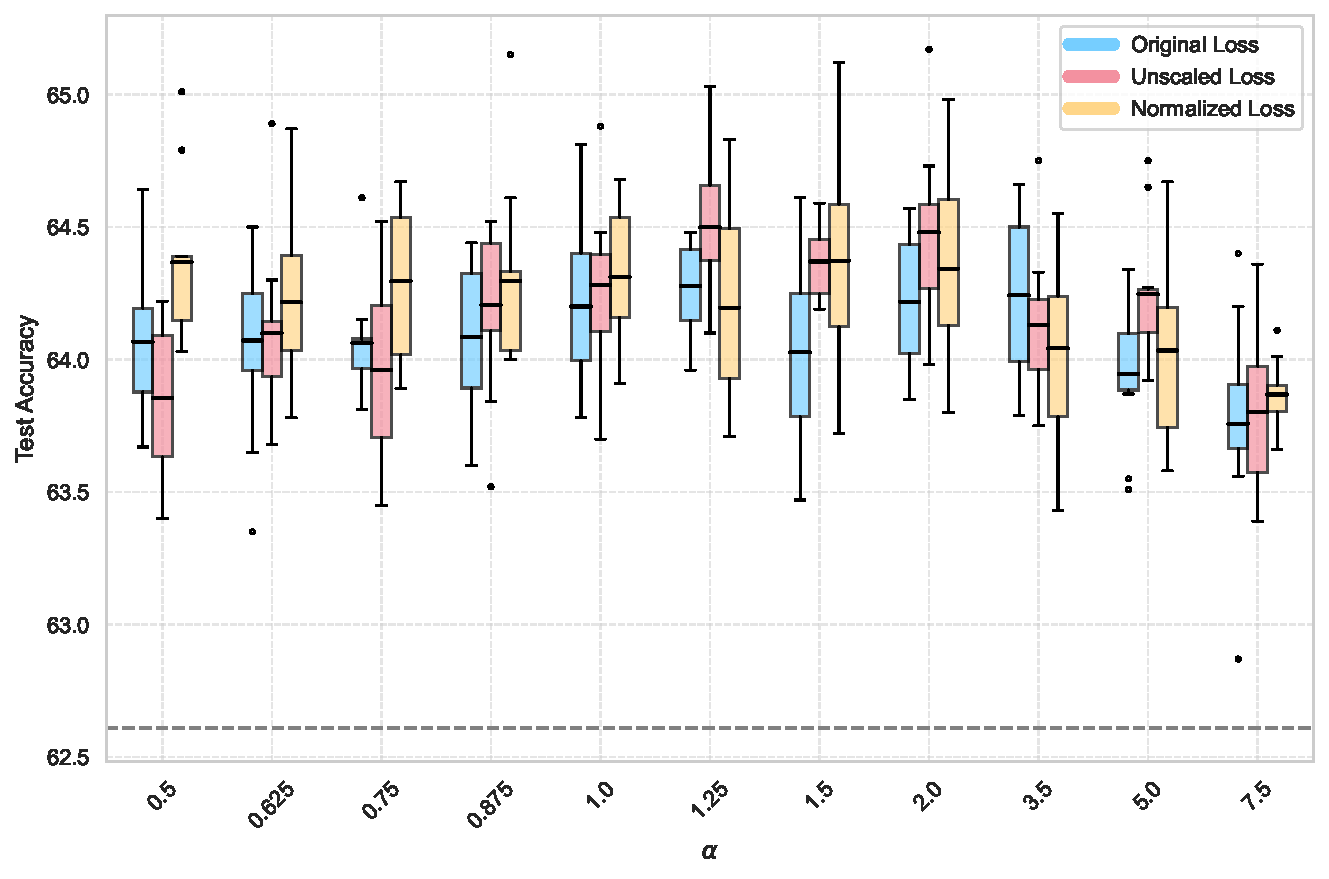
\includegraphics[width=0.7\textwidth]{../img/exp2_box_grouped_220.pdf}
	\caption{Boxplots of the performance of fully-trained models from Experiment 2, with mean values indicated by black lines and the performance of the vanilla model represented by a dashed gray line.}
	\label{fig:exp2_box_grouped_220}
\end{figure}

Figure~\ref{fig:exp2_box_grouped_220} shows the unaggregated results in the form of boxplots. From the figure, it is clear that the models utilizing the unscaled Rényi loss function achieve the best performance compared to the other approaches for $\alpha$ values between 1.25 and 2. Conversely, for $\alpha$ values below 0.75, these models perform the worst on average. For $\alpha$ greater than 3.5 the accuracy decreases across all models.

Interestingly, the performance of models using the normalized loss function remains relatively constant for all $\alpha$ values up to 3.5. Additionally, for all $\alpha$ values except 1.25, the average accuracy exceeds that of the student models trained with the original loss function.

Looking at Figure~\ref{fig:exp2_box_grouped_10}, which shows the performance of the models after only 10 out of 220 training epochs, we observe that the student models of the unscaled loss exhibit the most extreme behavior, achieving nearly 30\% accuracy for $\alpha \geq 3.5$, but failing to reach even 10\% for $\alpha=0.5$. This is most probably due to the difference in the gradients we have observed in Figure~\ref{fig:gradients_boxplot_noadj}. This, in turn, affects the effective learning rate, which then might result in lower performance of the models with low hyperparameter $\alpha$.

\begin{figure}[h!]
	\centering
	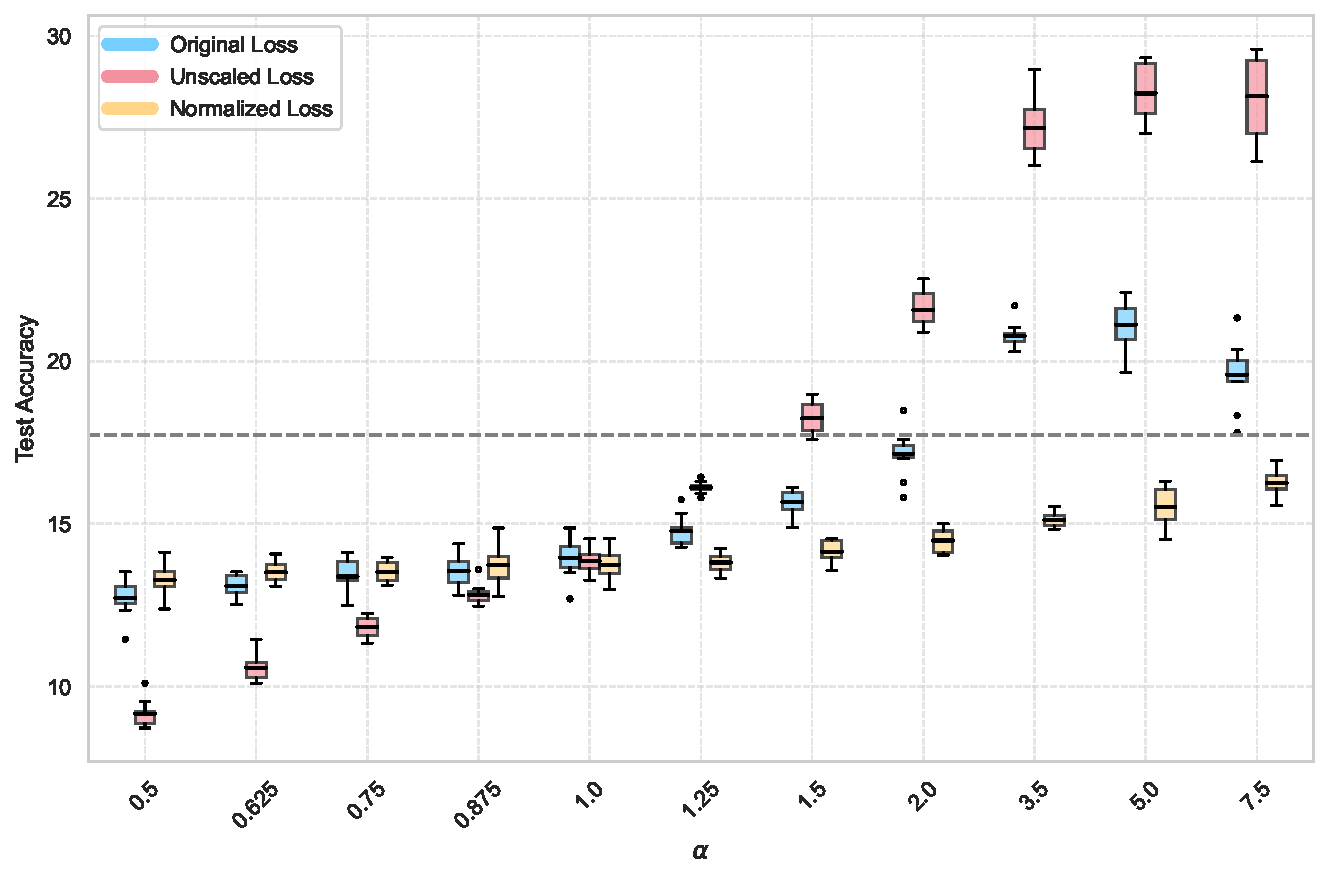
\includegraphics[width=0.7\textwidth]{../img/exp2_box_grouped_10.pdf}
	\caption{Boxplots of the performance of models from Experiment 2 after 10 epochs, with mean values indicated by black lines and the performance of the vanilla model represented by a dashed gray line.}
	\label{fig:exp2_box_grouped_10}
\end{figure}

Turning our attention to the student models trained with the normalized Rényi loss function, we observe that their performance remains much more consistent across different values of $\alpha$. However, there is still a difference, where the accuracy for $\alpha>3.5$ is around 15\% after 10 epochs, but only about 13\% for $\alpha=0.5$. This implies that higher $\alpha$ values improve performance early in training, not only by increasing the effective learning rate but also through other factors.

\begin{figure}[h!]
	\centering
	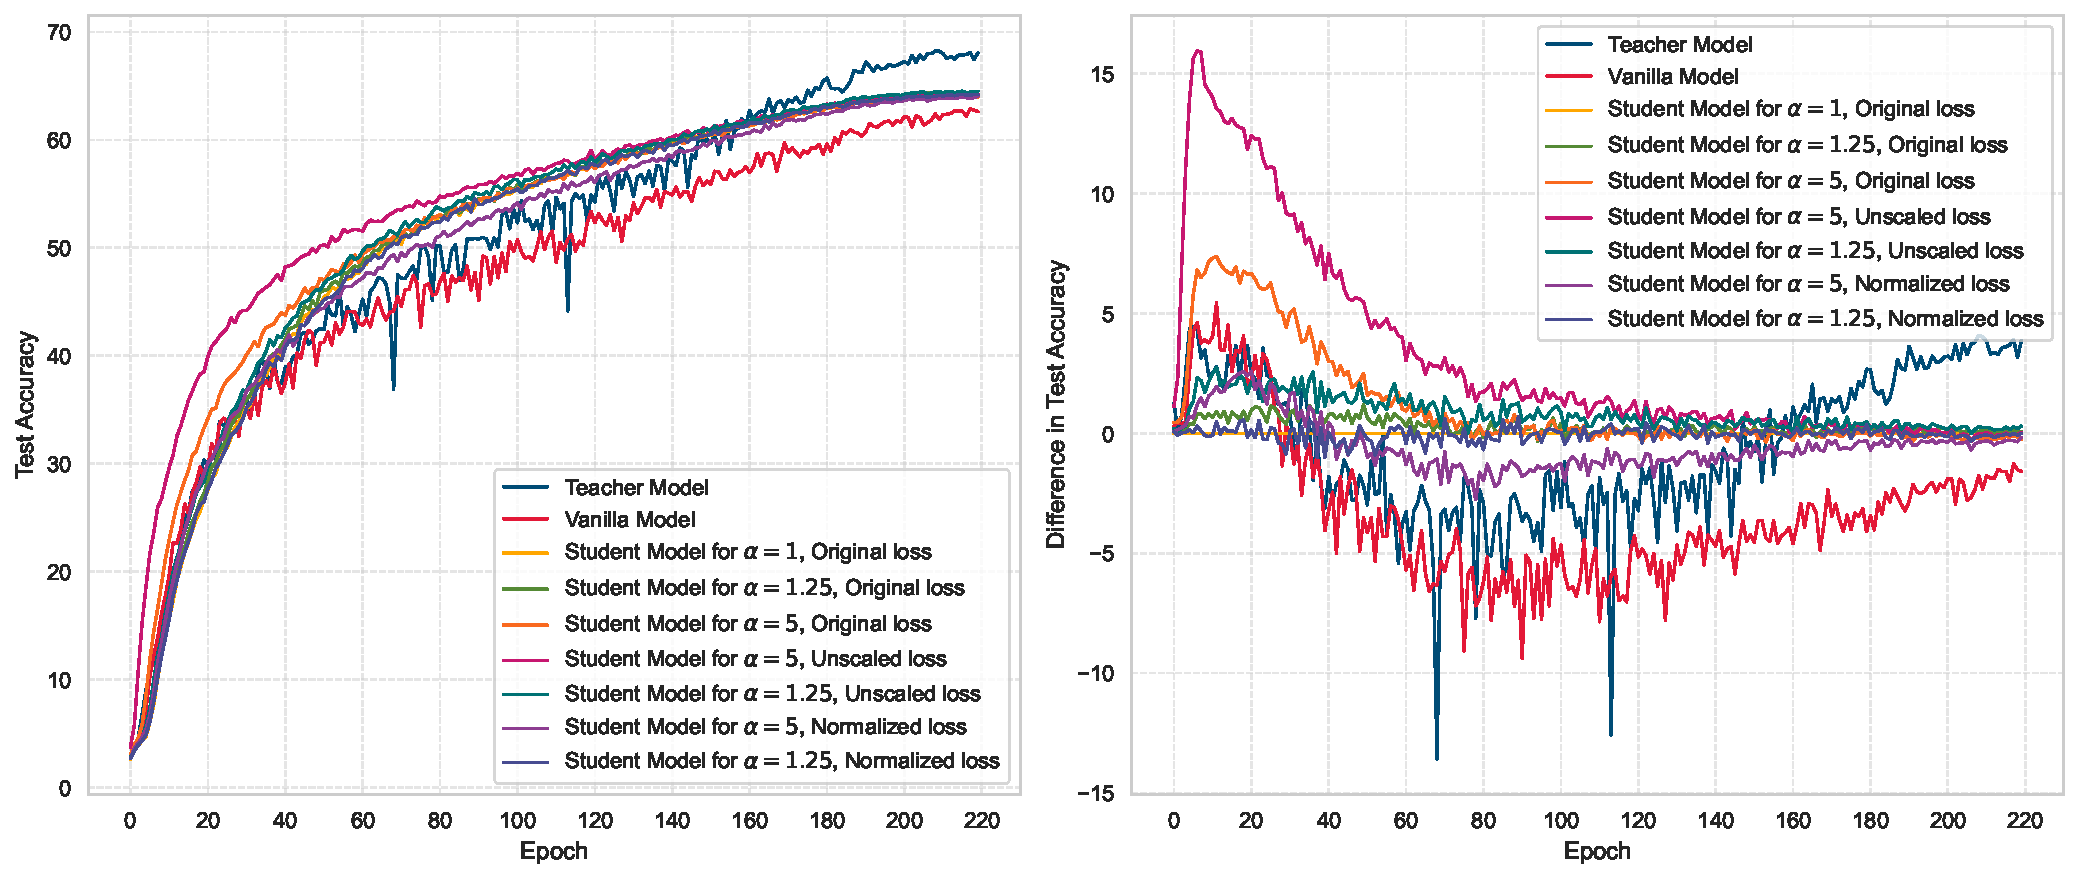
\includegraphics[width=1\textwidth]{../img/exp2_line_and_diff_plot.pdf}
	\caption{Comparison of the models with modified loss function. Left: Validation accuracy over 220 epochs for the teacher, vanilla, and selected student models. Right: Difference in accuracy compared to the student model with $\alpha=1$ over 220 epochs (Student models show averages over 10 iterations).}
	\label{fig:exp2_line_and_diff_plot}
\end{figure}

Lastly, Figure~\ref{fig:exp2_line_and_diff_plot} shows the performance of the various student models over the entire training process, rather than at a single epoch. Additionally, the plot on the right shows the difference in accuracy between these models and the student model trained with standard knowledge distillation.

We observe that models using the unscaled Rényi loss function with $\alpha = 5$ not only achieve the best performance at epoch 10, but also maintain this lead for a substantial portion of the training, remaining the top performers for approximately 120 epochs. This difference, when compared to the models trained with standard knowledge distillation, peaks around epoch 10, reaching approximately 15\%. When examining the models with the same loss function but using $\alpha = 1.25$, we observe that they outperform standard knowledge distillation during the initial epochs, though the difference is smaller, only about 2\%. This advantage gradually diminishes but remains noticeable until around epoch 120.

When comparing models trained with the unscaled loss to those using the original loss, we observe that the advantage over standard knowledge distillation peaks around the same epoch in both cases, but the gap is larger for the unscaled loss. Moreover, while the original loss shows a noticeable advantage for about 70 epochs, the unscaled version maintains this advantage for approximately 120 epochs.

On the other hand, the training process using the normalized loss behaves quite differently. For $\alpha = 1.25$, its behavior closely mirrors that of standard knowledge distillation, showing essentially no distinction. While for $\alpha = 5$, the normalized loss results in higher performance, with about 2\% better accuracy after 10 to 20 epochs. By epoch 40, the performances are nearly the same. However, after that point, the standard model begins to perform better, with the difference in accuracy reaching a peak of approximately 1\% around epoch 80. Although the gap becomes smaller again toward the end of training, the normalized model ultimately performs about 0.2\% worse.

\section{Discussion}

The first experiment confirmed the known benefits of knowledge distillation, which consistently outperformed the vanilla student model. More notably, models with values of $\alpha$ within the range of 1 to 3.5 produced better results than the standard knowledge distillation. However, these improvements were not statistically significant under conventional thresholds, and thus require further investigation through larger-scale experiments.

Interestingly, the early stages of training revealed a different dynamic. Higher values of $\alpha$ (e.g., 3.5 or 5) led to a higher test accuracy in the early stages of training. This suggests that larger values of $\alpha$ might be particularly useful in settings where early convergence or rapid experimentation is desirable. This advantage diminishes as training progresses and does not translate to better final performance.

In the second experiment, we proposed two alternatives to the Rényi loss function used in knowledge distillation, by modifying the scaling term, as we feared the higher performance in early stages was due to higher effective learning rate. Both strategies aimed to reduce this indirect influence of $\alpha$, either by applying a constant scaling across different values of $\alpha$ (unscaled Rényi loss function), or by adjusting it based on the behavior of the median of gradients (normalized Rényi loss function).

The results showed that the unscaled loss function slightly outperformed both the original and normalized versions, with the best performance achieved at $\alpha = 1.25$. The normalized version also surpassed the original and had consistent performance across all values of $\alpha$ between 0.5 and 3.5.

In the early stages, models with high $\alpha$ using the unscaled loss function performed best, which we attribute to their higher effective learning rate, as we observed that this approach does not normalize the means of the gradients. The performance advantage of models with high $\alpha$ using the unscaled normalized function was not as high, but it was still present, suggesting that higher values of $\alpha$ improve performance in the early phases of training, not only by increasing the effective learning rate.

Despite the promising results, it is important to stress that all testing was conducted on a small scale using the CIFAR-100 dataset. For a more conclusive evaluation of our proposed methods, we recommend testing on a much larger scale, such as with the ImageNet dataset (see \cite{Deng2009}).

Further research might also include tuning other introduced hyperparameters, such as $\beta$ and temperature $T$, in addition to standard hyperparameters like learning rate and weight decay. There may also be potential in creating a dynamic schedule for the hyperparameter $\alpha$, changing it during the training process for faster convergence and better performance. Calculating the function $\phi(\alpha,T)$ from Equation~\ref{modified_RL_sigmoid} for values of $T \neq 4$, or deriving an analytical solution, as well as focusing on the effect variance of gradients, which differs for various values of $\alpha$ and different Rényi loss functions, could be interesting directions for further work.









\chapter*{Conclusion}
\addcontentsline{toc}{chapter}{Conclusion}

This thesis focused on modifying knowledge distillation by replacing the Kullback-Leibler divergence (KL divergence) with Rényi divergence, introducing an additional hyperparameter $\alpha$, which increased the flexibility of the training process.

In the first chapter, we provided theoretical definitions of entropy, cross-entropy, Kullback-Leibler (KL) divergence, and Rényi divergence, together with an exploration of their relationship and the theoretical properties of Rényi divergence. We then introduced the concept of knowledge distillation and inspected key theoretical results. Finally, we replaced the KL divergence with Rényi divergence in the knowledge distillation framework and analyzed how some of the properties of Rényi divergence previously discussed affect the Rényi-based knowledge distillation, marking one of the key contributions of this thesis. 

The second chapter focused on the optimization of the previously defined Rényi-based knowledge distillation loss function using the stochastic gradient descent (SGD) algorithm. Additionally, we provided a detailed description of the Residual Neural Network (ResNet) architecture, including the neuron, ReLU activation function, convolutional layer, and residual block. Both SGD and ResNet were utilized in the subsequent chapter.

Arguably, the largest contribution of this thesis lies in the final chapter, which presents two experiments. In the first experiment we evaluated the effectiveness of Rényi-based knowledge distillation and compared it to the standard form of knowledge distillation. We observed promising improvements in model performance with $\alpha = 1.25$, and also identified significantly faster early convergence in models with higher values of the hyperparameter $\alpha$.

For the second experiment, we introduced two additional formulations of Rényi-based knowledge distillation, motivated by the effort of reducing the indirect influence of $\alpha$ on the learning rate. We also evaluated the performance of the new formulation, with the first one, utilizing unscaled Rényi loss, essentially amplified the results observed in the initial experiment but also magnified its shortcomings. The second formulation, which used the normalized Rényi loss function, also yielded promising results in terms of final accuracy, while overcoming the shortcomings of the previous formulations. We also observed notable convergence at the beginning of the training process, although it was considerably smaller in magnitude.

In the following discussion, we acknowledged the limitations of the thesis while also outlining potential avenues for future research in the area of Rényi-based knowledge distillation.


%%% Bibliography
%%% Bibliography (literature used as a source)
%%%
%%% We employ bibTeX to construct the bibliography. It processes
%%% citations in the text (e.g., the \cite{...} macro) and looks up
%%% relevant entries in the bibliography.bib file.
%%%
%%% The \bibliographystyle command selects, which style will be used
%%% for references from the text. The argument in curly brackets is
%%% the name of the corresponding style file (*.bst). Both styles
%%% mentioned in this template are included in LaTeX distributions.

\bibliographystyle{plainnat}    %% Author (year)
% \bibliographystyle{unsrt}     %% [number]

\renewcommand{\bibname}{Bibliography}

%%% Generate the bibliography. Beware that if you cited no works,
%%% the empty list will be omitted completely.

\bibliography{bibliography}

%%% If case you prefer to write the bibliography manually (without bibTeX),
%%% you can use the following. Please follow the ISO 690 standard and
%%% citation conventions of your field of research.

% \begin{thebibliography}{99}
%
% \bibitem{lamport94}
%   {\sc Lamport,} Leslie.
%   \emph{\LaTeX: A Document Preparation System}.
%   2nd edition.
%   Massachusetts: Addison Wesley, 1994.
%   ISBN 0-201-52983-1.
%
% \end{thebibliography}


%%% Figures used in the thesis (consider if this is needed)
\listoffigures

%%% Tables used in the thesis (consider if this is needed)
%%% In mathematical theses, it could be better to move the list of tables to the beginning of the thesis.
\listoftables

%%% Abbreviations used in the thesis, if any, including their explanation
%%% In mathematical theses, it could be better to move the list of abbreviations to the beginning of the thesis.
\chapwithtoc{List of Abbreviations}

%%% Attachments to the bachelor thesis, if any. Each attachment must be
%%% referred to at least once from the text of the thesis. Attachments
%%% are numbered.
%%%
%%% The printed version should preferably contain attachments, which can be
%%% read (additional tables and charts, supplementary text, examples of
%%% program output, etc.). The electronic version is more suited for attachments
%%% which will likely be used in an electronic form rather than read (program
%%% source code, data files, interactive charts, etc.). Electronic attachments
%%% should be uploaded to SIS and optionally also included in the thesis on a~CD/DVD.
%%% Allowed file formats are specified in provision of the rector no. 72/2017.
\appendix
\chapter{Attachments}

\section{First Attachment}

\openright
\end{document}
